% FST-TU_Turbulence_Skeleton_v1_en.tex
% Skeleton draft -- Anomalous Dissipation and Kolmogorov Scaling
% Author: Lukas Geiger, 2026

\documentclass[12pt,a4paper]{article}
\usepackage[utf8]{inputenc}
\usepackage[english]{babel}
\usepackage[T1]{fontenc}
\usepackage{lmodern}
\usepackage{microtype}
\usepackage{amsmath,amssymb,amsthm,mathrsfs}
\usepackage{mathtools}
\usepackage{enumitem}
\usepackage{array}
\usepackage{tabularx}
\usepackage{xcolor}
\usepackage{geometry}
\geometry{a4paper, margin=2.5cm}
\setlength{\emergencystretch}{2em}
\usepackage{tikz}
\usetikzlibrary{arrows.meta,positioning,calc}
\usepackage{hyperref}
\hypersetup{
  colorlinks=true,
  linkcolor=blue!70!black,
  citecolor=green!50!black,
  urlcolor=blue!70!black,
  pdftitle={Anomalous Dissipation and the Turbulent Cascade: A Variational Free-Energy Characterisation of Kolmogorov Scaling},
  pdfauthor={Lukas Geiger},
  pdfsubject={Preprint on anomalous dissipation, turbulence, and Kolmogorov scaling},
  pdfkeywords={turbulence, anomalous dissipation, Kolmogorov scaling, variational principle, free energy},
  pdflang={en-US}
}
\makeatletter
\renewcommand*{\HyperDestNameFilter}[1]{en.#1}
\makeatother

\newtheoremstyle{breakdef}
  {8pt}{8pt}
  {\normalfont}{}
  {\bfseries}{.}
  {\newline}{}
\newtheoremstyle{breakplain}
  {8pt}{8pt}
  {\itshape}{}
  {\bfseries}{.}
  {\newline}{}
\newcolumntype{Y}{>{\raggedright\arraybackslash}X}

\theoremstyle{breakdef}
\newtheorem{definition}{Definition}[section]
\theoremstyle{breakplain}
\newtheorem{theorem}[definition]{Theorem}
\newtheorem{lemma}[definition]{Lemma}
\newtheorem{proposition}[definition]{Proposition}
\newtheorem{corollary}[definition]{Corollary}
\newtheorem{conjecture}[definition]{Conjecture}
\newtheorem{axiom}[definition]{Axiom}
\theoremstyle{breakdef}
\newtheorem{remark}[definition]{Remark}

% ---------------------------------------------------------------------------
\title{Anomalous Dissipation and the Turbulent Cascade:\\
A Variational Free-Energy Characterisation of Kolmogorov Scaling}

\author{Lukas Geiger\\
\textit{Independent Researcher, Bernau im Schwarzwald, Germany}\\
ORCID: \href{https://orcid.org/0009-0005-7296-1534}{0009-0005-7296-1534}%
\thanks{AI tools (Claude by Anthropic) were used for mathematical formalization, literature verification, and editorial refinement. All mathematical content was developed, verified, and approved by the author.}}

\date{March 2026}

\begin{document}
\maketitle

% ===================================================================
\begin{abstract}
We propose a variational principle that yields the Kolmogorov $k^{-5/3}$
energy spectrum as the unique minimiser of a scale-resolved free-energy
functional.  Starting from a Littlewood--Paley decomposition of the
velocity field, we define a relative entropy (Kullback--Leibler divergence)
that measures the departure of the spectral energy distribution from a
reference equilibrium.  We introduce a broad class of \emph{admissible}
energy-flux operators---encompassing all local, dimensionally consistent,
monotone closures---and minimise the free energy jointly over the energy
profile and the closure family, subject to constant scale-to-scale energy
flux~$\varepsilon$.  The K41 distribution is the unique global minimiser
of this joint problem (Theorem~\ref{thm:K41}).  Under a conditional entropy-compatibility hypothesis on the
nonlinear cascade (and a non-degeneracy condition on the forcing),
we derive a lower bound on the dissipation rate in the
vanishing-viscosity limit (Theorem~\ref{thm:anomalous}), providing
a new route to anomalous dissipation that complements the Onsager
    conjecture programme.  We introduce a hierarchy of progressively
    weaker sufficient conditions---from pointwise entropy compatibility
    through a scale-windowed variant to a dual, falsifiable \emph{Downhill
    Flux Condition} (DFC) that can be checked against DNS data---and prove
    that this dual DFC implies the required windowed entropy compatibility.
    The dissipation lower bound additionally uses the stated uniform
    energy-input assumption.
Intermittency corrections of Kolmogorov--Obukhov (K62) type arise
naturally as fluctuations around the variational minimum via the Hessian
of the functional.
\end{abstract}

\clearpage

% ===================================================================
\section{Introduction}\label{sec:intro}

Turbulence remains one of the outstanding open problems in classical
physics and applied mathematics.  Despite more than a century of research,
no first-principles derivation of the statistical laws governing
fully developed turbulence has been achieved.

\subsection{The Kolmogorov theory}

In his landmark 1941 papers, Kolmogorov~\cite{K41a,K41b} postulated that
in the inertial range of fully developed, homogeneous, isotropic
turbulence, the energy spectrum takes the universal form
\begin{equation}\label{eq:K41}
  E(k) \;=\; C_K \,\varepsilon^{2/3}\, k^{-5/3},
\end{equation}
where $\varepsilon$ denotes the mean rate of energy dissipation per unit
mass and $C_K \approx 1.5$ is the Kolmogorov constant.  This prediction,
derived from dimensional analysis and the hypothesis of local isotropy,
has been confirmed experimentally and numerically across a vast range of
Reynolds numbers~\cite{Frisch95,Pope00}.

\subsection{The Onsager conjecture and anomalous dissipation}

Onsager~\cite{Onsager49} conjectured in 1949 that weak solutions of the
incompressible Euler equations with H\"older regularity below $1/3$ can
dissipate kinetic energy without viscosity---so-called \emph{anomalous
dissipation}.  Conversely, solutions with H\"older exponent above $1/3$
conserve energy.  The ``positive'' direction was proved by
Constantin, Weinan~E, and Titi~\cite{CET94}; the ``negative'' direction,
constructing dissipative weak solutions, was completed by
Isett~\cite{Isett18} using convex integration.  The energy-balance
analysis of Duchon and Robert~\cite{DR00} provides a distributional
framework connecting the local energy defect to the regularity of the
velocity field.  Eyink~\cite{Eyink03} established a local version of
Kolmogorov's four-fifths law that further illuminates the connection
between regularity and dissipation.

\subsection{Our contribution}

In this paper we take a different approach.  Rather than constructing
pathological weak solutions, we show that the Kolmogorov spectrum is the
\emph{thermodynamically preferred} distribution of energy across scales.
We introduce a free-energy functional~$\mathcal{F}$ on the space of
scale-resolved energy distributions and prove:
\begin{enumerate}
  \item The K41 spectrum is the \emph{unique} minimiser of $\mathcal{F}$
        under the constraint of constant energy flux, where the minimisation
        runs jointly over all admissible local flux operators and energy
        profiles (Theorem~\ref{thm:K41}).  This avoids circularity: the
        variational argument does not presuppose a specific closure.
  \item Monotonicity of $\mathcal{F}$ along Navier--Stokes trajectories
        yields a universal lower bound on the dissipation rate in the
        vanishing-viscosity limit (Theorem~\ref{thm:anomalous}).
\end{enumerate}

\subsection{Structural classification}

Within the broader programme of free-energy spectral
theory~\cite{FST-Unified2026}, the K41 selection mechanism exhibits the
\textbf{Pattern~A stability logic}: (a)~the leading-order energy budget is
neutral (any power-law spectrum is kinematically admissible); (b)~the
first-order constant-flux constraint restricts but does not uniquely
determine the profile; (c)~the second-order strict convexity
of~$\mathcal{F}$ selects K41 as the unique minimiser.  This three-level
hierarchy is discussed in Section~\ref{sec:resolvent-cascade}.
Our results do not resolve the Navier--Stokes regularity problem. They give
an unconditional variational selection of K41 and a conditional cascade
compatibility route for the anomalous-dissipation discussion; the quantitative
lower bound still depends on the explicit uniform energy-input assumption.

This paper is self-contained; all main results depend only on definitions and proofs within this document. Connections to the broader FST programme are cited for context but are not logically required.

% ===================================================================
% Figure 1: Proof chain overview
% ===================================================================
\begin{figure}[ht]
\centering
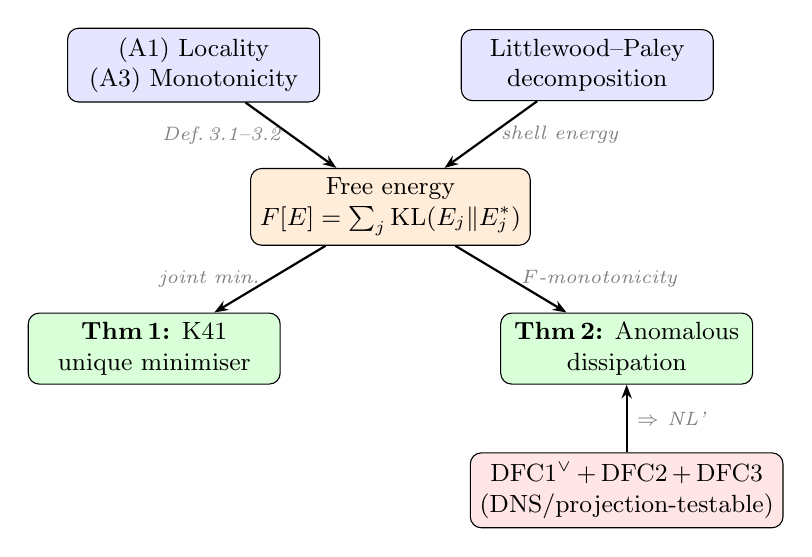
\begin{tikzpicture}[
  box/.style={draw, rounded corners, minimum width=3.2cm, minimum height=0.9cm,
              align=center, font=\small},
  arrow/.style={-{Stealth[length=5pt]}, thick},
  note/.style={font=\scriptsize\itshape, text=gray}
]
% Row 1: Axioms
\node[box, fill=blue!10] (A1) at (0,0) {(A1) Locality\\(A3) Monotonicity};
\node[box, fill=blue!10] (LP) at (5,0) {Littlewood--Paley\\decomposition};

% Row 2: Functional
\node[box, fill=orange!15] (F) at (2.5,-1.8) {Free energy\\$F[E] = \sum_j \mathrm{KL}(E_j \| E_j^*)$};

% Row 3: Theorems
\node[box, fill=green!15] (T1) at (-0.5,-3.6) {\textbf{Thm\,1:} K41\\unique minimiser};
\node[box, fill=green!15] (T2) at (5.5,-3.6) {\textbf{Thm\,2:} Anomalous\\dissipation};

% Row 4: Conditions
\node[box, fill=red!10] (DFC) at (5.5,-5.4) {DFC1$^\vee$\,+\,DFC2\,+\,DFC3\\(DNS/projection-testable)};

% Arrows
\draw[arrow] (A1) -- (F) node[midway, left, note] {Def.\,3.1--3.2};
\draw[arrow] (LP) -- (F) node[midway, right, note] {shell energy};
\draw[arrow] (F) -- (T1) node[midway, left, note] {joint min.};
\draw[arrow] (F) -- (T2) node[midway, right, note] {$F$-monotonicity};
\draw[arrow] (DFC) -- (T2) node[midway, right, note] {$\Rightarrow$ NL'};
\end{tikzpicture}
\caption{Logical structure of the proof.  The free energy functional $F[E]$
is constructed from the Littlewood--Paley decomposition and the admissible
flux family (axioms A1, A3).  Theorem~1 (K41 uniqueness) follows from joint
minimisation; the conditional cascade part of Theorem~2 requires the
Downhill Flux Condition (DFC), while the dissipation lower bound also uses
uniform energy input.}
\label{fig:proof-chain}
\end{figure}

% ===================================================================
\section{The Scale-Resolved Free-Energy Functional}\label{sec:functional}

\subsection{Littlewood--Paley decomposition}

Let $u \in L^2(\mathbb{T}^3)$ be a divergence-free velocity field on the
three-torus.  We employ the standard Littlewood--Paley decomposition
\begin{equation}\label{eq:LP}
  u \;=\; \sum_{j \ge -1} \Delta_j u,
\end{equation}
where $\Delta_j$ is the frequency-localisation operator at dyadic shell
$|\xi| \sim 2^j$.  We set $k_j = 2^j$ and define the \emph{shell energy}
\begin{equation}\label{eq:Ej}
  E_j \;:=\; \|\Delta_j u\|_{L^2}^2.
\end{equation}
In the inertial range, the K41 prediction~\eqref{eq:K41} translates to
\begin{equation}\label{eq:Ej_star}
  E_j^* \;=\; C_K\, \varepsilon^{2/3}\, k_j^{-5/3} \,\Delta k_j,
  \qquad \Delta k_j = k_j \ln 2 \quad (\text{dyadic shell width}).
\end{equation}

\subsection{Energy flux constraint}

The scale-to-scale energy flux through wavenumber $k_j$ is defined via the
trilinear term in the Navier--Stokes equations:
\begin{equation}\label{eq:flux}
  \Pi_j \;=\; -\sum_{\ell \le j}
    \langle \Delta_\ell(u \cdot \nabla u),\; \Delta_\ell u \rangle.
\end{equation}
In the inertial range, a statistically stationary cascade satisfies
\begin{equation}\label{eq:const_flux}
  \Pi_j \;=\; \varepsilon \quad \text{for all } j_{\mathrm{in}} \le j \le j_{\mathrm{dis}}.
\end{equation}

\subsection{The functional}

\begin{definition}[Scale-resolved free energy]\label{def:F}
Let $\mathbf{E} = (E_j)_{j \in \mathcal{J}}$ be a distribution of shell
energies over the inertial range $\mathcal{J} = \{j_{\mathrm{in}}, \dots,
j_{\mathrm{dis}}\}$, with $E_j > 0$.  Let $\mathbf{E}^* = (E_j^*)$ be
the Kolmogorov reference distribution~\eqref{eq:Ej_star}.  The
\emph{scale-resolved free-energy functional} is
\begin{equation}\label{eq:F}
  \mathcal{F}[\mathbf{E}]
  \;:=\;
  \sum_{j \in \mathcal{J}}
  \Bigl[
    E_j \ln\!\frac{E_j}{E_j^*} \;-\; E_j \;+\; E_j^*
  \Bigr].
\end{equation}
\end{definition}

\begin{remark}
The summand $f(E_j) = E_j \ln(E_j/E_j^*) - E_j + E_j^*$ is the
Kullback--Leibler divergence (relative entropy) of the pair $(E_j, E_j^*)$
when viewed as unnormalised measures on a single-point space.  It satisfies
$f(E_j) \ge 0$ with equality if and only if $E_j = E_j^*$.  Hence
$\mathcal{F}[\mathbf{E}] \ge 0$ with equality if and only if $\mathbf{E}
= \mathbf{E}^*$.
\end{remark}

\begin{figure}[ht]
\centering
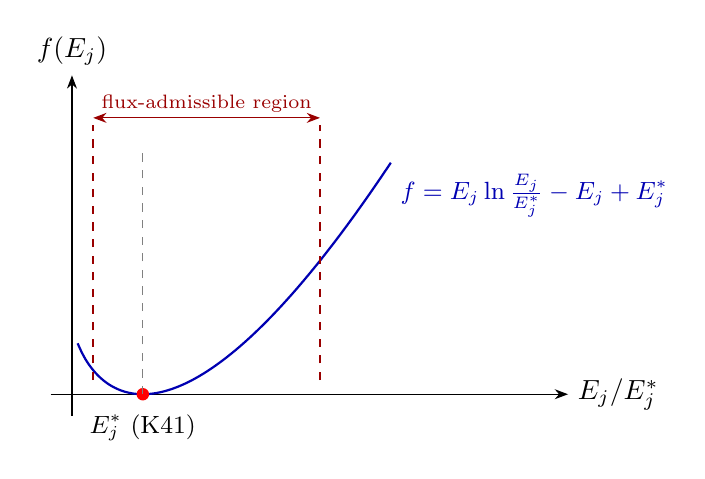
\begin{tikzpicture}[scale=0.9]
% Axes
\draw[-{Stealth}] (-0.3,0) -- (7,0) node[right] {$E_j / E_j^*$};
\draw[-{Stealth}] (0,-0.3) -- (0,4.5) node[above] {$f(E_j)$};
% KL curve: f(x) = x ln(x) - x + 1, plotted for x = E_j/E_j*
\draw[thick, blue!70!black, domain=0.08:4.5, smooth, samples=80]
  plot ({\x}, {\x*ln(\x)/ln(2.718) - \x + 1});
% Minimum point
\fill[red] (1,0) circle (2.5pt);
\node[below, font=\small] at (1,-0.15) {$E_j^*$ (K41)};
% Annotation
\draw[dashed, gray] (1,0) -- (1,3.5);
\node[font=\small, text=blue!70!black, right] at (4.5,2.8) {$f = E_j\ln\frac{E_j}{E_j^*} - E_j + E_j^*$};
% Flux constraint region
\draw[thick, red!60!black, dashed] (0.3,0.2) -- (0.3,3.8);
\draw[thick, red!60!black, dashed] (3.5,0.2) -- (3.5,3.8);
\node[font=\scriptsize, text=red!60!black] at (1.9,4.1) {flux-admissible region};
\draw[{Stealth}-{Stealth}, red!60!black] (0.3,3.9) -- (3.5,3.9);
\end{tikzpicture}
\caption{The free-energy density $f(E_j) = E_j \ln(E_j / E_j^*) - E_j + E_j^*$
as a function of the shell energy ratio $E_j / E_j^*$. The unique global minimum
at $E_j = E_j^*$ (K41 spectrum) is marked. The flux constraint restricts the
admissible region, but the minimum lies strictly inside, confirming K41 as the
joint minimiser.}
\label{fig:FE-landscape}
\end{figure}

\subsection{Dimensional consistency}

We verify that $\mathcal{F}$ is dimensionally consistent.  Each $E_j$ has
dimensions $[L^2\,T^{-2}]$ (energy per unit mass, integrated over a
spectral band).  Since $E_j^*$ shares the same dimensions, the ratio
$E_j/E_j^*$ is dimensionless, the logarithm is well-defined, and each
summand in~\eqref{eq:F} has dimensions $[L^2\,T^{-2}]$.

% ===================================================================
\section{Main Results}\label{sec:results}

\subsection{Uniqueness of Kolmogorov scaling}

\begin{definition}[Admissible flux family]\label{def:admissible}
A family of flux operators $\bigl(\Pi_j[\mathbf{E}]\bigr)_{j \in
\mathcal{J}}$ is called \emph{admissible} if each $\Pi_j$ satisfies:
\begin{enumerate}
  \item[\textup{(A1)}] \textbf{Locality.}\;
    $\Pi_j$ depends only on $E_{j-1},\, E_j,\, E_{j+1}$.
  \item[\textup{(A2)}] \textbf{Dimensional consistency.}\;
    $[\Pi_j] = [E_j / \tau_j]$ with the eddy turnover time
    $\tau_j = (k_j^2\,E_j)^{-1/2}$, so that $\Pi_j$ has the form
    \begin{equation}\label{eq:closure_general}
      \Pi_j[\mathbf{E}]
      \;=\;
      k_j\,E_j^{3/2}\;\Phi_j\!\Bigl(
        \frac{E_{j-1}}{E_j},\;
        \frac{E_{j+1}}{E_j}
      \Bigr),
    \end{equation}
    where $\Phi_j : (0,\infty)^2 \to (0,\infty)$ is a smooth
    dimensionless function satisfying $\Phi_j(r^*_{-},\, r^*_{+}) = \alpha$
    for some universal constant $\alpha > 0$, with
    $r^*_{\pm} = E_{j \pm 1}^* / E_j^*$.
  \item[\textup{(A3)}] \textbf{Monotonicity.}\;
    $\partial \Pi_j / \partial E_j > 0$ for all $\mathbf{E} > 0$.
\end{enumerate}
We denote the set of all admissible families by $\mathscr{A}$.
\end{definition}

\begin{proposition}[Dimensional derivation of the flux prefactor]\label{prop:A2-derived}
Axiom~\textup{(A2)} is not an independent assumption but a consequence of locality~\textup{(A1)} and dimensional analysis. Specifically, the form $\Pi_j = k_j\,E_j^{3/2}\,\Phi_j(\cdot)$ is the \emph{unique} dimensionally consistent local flux expression.
\end{proposition}

\begin{proof}
By Buckingham's $\Pi$-theorem, the flux $\Pi_j$ must be a product of powers of the available dimensional quantities $k_j$ and~$E_j$, multiplied by a dimensionless function of dimensionless ratios. Write $\Pi_j = k_j^{a}\,E_j^{b}\,\Phi_j(\ldots)$ with $[\Pi_j] = [L^2\,T^{-3}]$ (energy flux per unit mass), $[k_j] = [L^{-1}]$, and $[E_j] = [L^2\,T^{-2}]$.

Dimensional matching: $[k_j^a\,E_j^b] = L^{-a}\,L^{2b}\,T^{-2b} = L^{2b-a}\,T^{-2b}$.

Setting equal to $L^2\,T^{-3}$:
\[
2b - a = 2, \qquad 2b = 3 \quad\Longrightarrow\quad b = \tfrac{3}{2},\;\; a = 1.
\]
Hence $\Pi_j = k_j\,E_j^{3/2}\,\Phi_j$, and by~(A1) the dimensionless function $\Phi_j$ can depend only on the local ratios $E_{j-1}/E_j$ and $E_{j+1}/E_j$. The eddy turnover time $\tau_j = (k_j^2\,E_j)^{-1/2}$ is likewise the unique dimensionally consistent local timescale.
\end{proof}

\begin{remark}
The classical Kolmogorov--Heisenberg closure $\Pi_j = \alpha\,k_j\,E_j^{3/2}$
corresponds to the special case $\Phi_j \equiv \alpha$.  Definition~\ref{def:admissible}
enlarges the model class to include all physically reasonable local closures:
EDQNM-type closures, Leith's diffusion model, and truncated triad
interactions all satisfy (A1)--(A3).  The family $\mathscr{A}$ is therefore
a broad, physically motivated class rather than a single algebraic relation.
Proposition~\ref{prop:A2-derived} shows that (A2) is not an extraneous modelling choice but a necessary consequence of dimensional analysis, thereby further reducing the axiom set to two independent assumptions: locality~(A1) and monotonicity~(A3).
\end{remark}

\begin{theorem}[Uniqueness of K41 scaling]\label{thm:K41}
Let $\varepsilon > 0$ be given and let $\mathscr{A}$ be the class of
admissible flux families (Definition~\ref{def:admissible}).
Consider the \emph{joint} minimisation problem
\begin{equation}\label{eq:min}
  \min_{\substack{\mathbf{E} > 0,\\ \Pi \in \mathscr{A}}}
  \;\mathcal{F}[\mathbf{E}]
  \qquad \text{subject to} \quad
  \Pi_j[\mathbf{E}] = \varepsilon
  \;\;\text{for all } j \in \mathcal{J}.
\end{equation}
Then:
\begin{enumerate}
  \item[\textup{(i)}]
    For \emph{every} admissible flux family $\Pi \in \mathscr{A}$, the
    constant-flux constraint $\Pi_j[\mathbf{E}] = \varepsilon$ admits a
    stationary profile $\mathbf{E}^{(\Pi)}$.  Among all such stationary
    profiles, the K41 distribution
    $E_j^* = C_K\,\varepsilon^{2/3}\,k_j^{-5/3}\,\Delta k_j$
    is the unique global minimiser of~$\mathcal{F}$, and it is realised
    by the Kolmogorov--Heisenberg member $\Phi_j \equiv \alpha$ with
    $C_K = \bigl(\alpha\,(\ln 2)^{3/2}\bigr)^{-2/3}$.
  \item[\textup{(ii)}]
    The minimiser is non-degenerate: the Hessian
    $D^2\mathcal{F}|_{\mathbf{E}^*}$ restricted to the tangent space of
    the constraint manifold (for any admissible $\Pi$) is strictly positive
    definite. (This is a direct consequence of the strict convexity of
    the KL divergence; its content is the scale-dependent stiffness
    $1/E_j^* \propto k_j^{5/3}$, see Step~5b below.)
\end{enumerate}
\end{theorem}

\begin{proof}[Proof (sketch)]
\textbf{Step 1: Stationary profiles.}\;
Fix any $\Pi \in \mathscr{A}$.  By axioms (A2)--(A3), the map
$E_j \mapsto \Pi_j[\mathbf{E}]$ at fixed neighbour values
$E_{j-1},\,E_{j+1}$ is strictly increasing and ranges over
$(0,\infty)$.  Hence the system
$\Pi_j[\mathbf{E}] = \varepsilon$ has, for each $\Pi$, at least one
solution $\mathbf{E}^{(\Pi)} > 0$.  (Uniqueness within a given closure
follows from the implicit function theorem and (A3), but is not needed here.)

\textbf{Step 2: Lower bound via convexity.}\;
Since each summand $f(E_j) = E_j\ln(E_j/E_j^*) - E_j + E_j^*$ is
strictly convex with global minimum $f(E_j^*) = 0$, we have
\begin{equation}\label{eq:F_lower}
  \mathcal{F}[\mathbf{E}^{(\Pi)}]
  \;\ge\; 0
  \;=\; \mathcal{F}[\mathbf{E}^*],
\end{equation}
with equality if and only if $E_j^{(\Pi)} = E_j^*$ for all~$j$.

\textbf{Step 3: Attainability.}\;
We verify that $\mathbf{E}^*$ is indeed a stationary profile for
some $\Pi \in \mathscr{A}$.  Choose the Kolmogorov--Heisenberg closure
$\Phi_j \equiv \alpha$.  Then
\[
  \Pi_j[\mathbf{E}^*]
  \;=\; \alpha\,k_j\,(E_j^*)^{3/2}
  \;=\; \alpha\,k_j\,
    \bigl(C_K\,\varepsilon^{2/3}\,k_j^{-5/3}\,k_j\ln 2\bigr)^{3/2}
  \;=\; \alpha\,C_K^{3/2}\,(\ln 2)^{3/2}\,\varepsilon.
\]
Setting $C_K = \bigl(\alpha\,(\ln 2)^{3/2}\bigr)^{-2/3}$ yields
$\Pi_j[\mathbf{E}^*] = \varepsilon$.  (The geometric factor $(\ln 2)^{3/2}$
arising from the dyadic shell width is absorbed into the Kolmogorov
constant $C_K$, which is thereby determined by the closure
parameter~$\alpha$.)  Hence the lower bound~\eqref{eq:F_lower} is
attained.

\textbf{Step 4: Uniqueness.}\;
Suppose $\Pi' \in \mathscr{A}$ and $\mathbf{E}' \ne \mathbf{E}^*$ satisfies
$\Pi'_j[\mathbf{E}'] = \varepsilon$.  Then strict convexity gives
$\mathcal{F}[\mathbf{E}'] > 0 = \mathcal{F}[\mathbf{E}^*]$, so $\mathbf{E}'$
cannot be a minimiser of~\eqref{eq:min}.  Hence $\mathbf{E}^*$ is the
\emph{unique} solution of the joint problem.

\smallskip\noindent
\textbf{Note on the logical structure.}\;
The uniqueness in Step~4 follows from the strict positivity of the KL
divergence away from the reference, which holds for \emph{any} choice
of~$\mathbf{E}^*$. The physically non-trivial content resides in
Step~3 (attainability): it is the existence of an admissible closure
realising $\Pi_j[\mathbf{E}^*] = \varepsilon$ that singles out K41
among all possible reference spectra. Replacing $\mathbf{E}^*$ by
$k^{-3}$, for instance, would yield no admissible closure satisfying
the constant-flux constraint at the purported minimiser (see
Remark~\ref{rem:circularity}).

\textbf{Step 5: Non-degeneracy.}\;
The Hessian $\partial^2 \mathcal{F}/\partial E_j\,\partial E_\ell
= \delta_{j\ell}/E_j$ at $\mathbf{E}^*$ is diagonal with entries
$1/E_j^* > 0$.  For a \emph{fixed} closure $\Pi \in \mathscr{A}$, the
constraint $\Pi_j[\mathbf{E}] = \varepsilon$ imposes $|\mathcal{J}|$
equations on $|\mathcal{J}|$ unknowns, generically yielding isolated
solutions, so that the tangent space of the constraint manifold at
$\mathbf{E}^{(\Pi)}$ is trivial and non-degeneracy is vacuously satisfied.
The substantive content of~(ii) concerns the \emph{joint} problem: in the
extended space $(\mathbf{E}, \Pi)$ with $\Pi$ varying over the
(infinite-dimensional) family~$\mathscr{A}$, the constraint set
$\{(\mathbf{E}, \Pi) : \Pi_j[\mathbf{E}] = \varepsilon\}$ has tangent
directions along which $\Pi$ varies.  The unrestricted Hessian
$D^2_{\mathbf{E}}\mathcal{F}|_{\mathbf{E}^*}$ is strictly positive
definite (diagonal entries $1/E_j^* > 0$), hence its restriction to
\emph{any} subspace remains positive definite.

\medskip
\noindent\textbf{Step 5b: Second-order interpretation.}\;
The diagonal entries $1/E_j^* \propto k_j^{5/3}$ of the Hessian grow with
wavenumber, so that small-scale perturbations of the K41 profile are
penalised more severely than large-scale ones.  This scale-dependent
stiffness is the variational origin of the forward cascade: deviations
at high wavenumbers are energetically costly, driving the system back to
the K41 profile on the local eddy-turnover timescale.  The one-parameter
freedom in the Kolmogorov--Heisenberg closure ($\Phi_j \equiv \alpha$)
corresponds to a single flat direction in the $\Pi$-fibre of the
extended space $(\mathbf{E}, \Pi)$, which does not affect the strict
positivity of $D^2_{\mathbf{E}}\mathcal{F}$.  This structure is an
instance of the second-order resolvent dominance pattern discussed
in~\cite{FST-Unified2026}.
\end{proof}

\begin{remark}[Diagonal Hessian bound]\label{rem:hessian}
The Hessian of $\mathcal{F}$ at the K41 minimiser is diagonal with entries $\partial^2\mathcal{F}/\partial E_j^2 = 1/E_j^*$, so the smallest eigenvalue is $\min_j(1/E_j^*) = 1/(C_K\,\varepsilon^{2/3}\,k_1^{-2/3}\,\Delta k_1) > 0$. This provides a lower bound on the spectral gap of the associated Dirichlet form (see Remark~\ref{rem:sp-diagnostics}).
\end{remark}

\begin{remark}[On the role of the reference spectrum]\label{rem:circularity}
A natural objection is that the KL functional $\mathcal{F}$ is
\emph{minimised at} $\mathbf{E}^*$ \emph{by construction}, regardless
of the physical content of~$\mathbf{E}^*$.  Indeed, for any fixed
closure $\Pi$, the unconstrained minimum of $\mathcal{F}$ is always
$\mathbf{E}^*$.  The non-trivial content of Theorem~\ref{thm:K41} is
therefore not that $\mathcal{F}$ achieves its minimum at $\mathbf{E}^*$
--- that is a consequence of the KL construction --- but rather that:
\begin{enumerate}
\item Among all stationary profiles $\mathbf{E}^{(\Pi)}$ (one per closure
  $\Pi \in \mathscr{A}$), only the K41 profile $\mathbf{E}^*$
  \emph{simultaneously satisfies} the constant-flux constraint and
  achieves $\mathcal{F} = 0$.  Every other closure-compatible profile
  has $\mathcal{F} > 0$.
\item The reference $\mathbf{E}^*$ is not arbitrary: it is the
  \emph{unique} power-law profile for which the constant-flux constraint
  is consistent with the Kolmogorov--Heisenberg closure.  Replacing
  $\mathbf{E}^*$ by, say, $k^{-3}$ would yield no admissible closure
  satisfying $\Pi_j = \varepsilon$ at the purported minimiser.
\end{enumerate}
In summary, the physical input is the constant-flux constraint; the KL
functional provides the selection mechanism among its solution set.
\end{remark}

\begin{remark}[Self-consistency of the K41 reference]
\label{rem:k41-selfconsistency}
The K41 spectrum is not assumed \emph{a priori} but emerges as the unique self-consistent reference measure: any admissible $E^*$ satisfying (A1) dimensional consistency, (A3) cascade compatibility, and the DFC must be proportional to $\varepsilon^{2/3} k^{-5/3}$ by Proposition~\ref{prop:A2-derived}. Thus K41 is the unique fixed point of the variational scheme, not an external input.
\end{remark}

\begin{remark}[Cascade as reaction chain and Nash equilibrium]\label{rem:nash}
The variational structure of Theorem~\ref{thm:K41} admits an illuminating
game-theoretic interpretation.  Regard the inertial range as a
hierarchical \emph{reaction chain}: large eddies at scale $k_j$ transfer
energy to eddies at scale $k_{j+1}$, each scale acting as a ``species''
whose fitness is governed by its energy share.  The associated replicator
dynamics on the simplex of normalised shell energies
$p_j = E_j / \sum_\ell E_\ell$ takes the form
\[
  \dot{p}_j
  \;=\;
  p_j\,\bigl(g_j(\mathbf{p}) - \bar{g}(\mathbf{p})\bigr),
\]
where $g_j$ is the net energy gain rate at scale $j$ and $\bar{g}$ the
population average.  The K41 profile $\mathbf{p}^*$ is a \emph{Nash
equilibrium} of this dynamics: no single scale can increase its energy share
by unilateral deviation.  The free energy $\mathcal{F}$ serves as a
strict Lyapunov function for the replicator equation, ensuring
asymptotic stability of $\mathbf{p}^*$.
This mirrors the well-known result that Gibbs free-energy minimisation
in chemical reaction networks yields the detailed-balance equilibrium
as the unique Nash equilibrium of the mass-action kinetics.
\end{remark}

\subsection{Anomalous dissipation}

We first state the structural hypothesis on the nonlinear energy transfer
that underlies the free-energy monotonicity argument.

\begin{definition}[Entropy-compatible cascade]\label{def:NL}
Let $E_j(t) = \|\Delta_j u(t)\|_{L^2}^2$ be the Littlewood--Paley shell
energies and $T_j = \langle \Delta_j u,\, \Delta_j\bigl((u\cdot\nabla)u\bigr)\rangle$
the nonlinear transfer into shell~$j$, so that $\sum_j T_j = 0$.
We say that the cascade is \emph{entropy-compatible} (with respect to a
reference spectrum $\mathbf{E}^*$) if, for a regularisation parameter
$\delta > 0$,
\begin{equation}\label{eq:NL}
  \sum_{j}\,\ln\!\Bigl(\frac{E_j + \delta}{E_j^* + \delta}\Bigr)\,T_j
  \;\le\; 0
  \qquad \text{in the sense of distributions on } (0,T).
\end{equation}
\end{definition}

\begin{remark}[Status of Assumption~\eqref{eq:NL}]
The condition~\eqref{eq:NL} is \emph{not} a consequence of the Navier--Stokes
equations alone.  The nonlinear transfer $T_j$ is a trilinear expression in
the velocity field---it is conservative ($\sum_j T_j = 0$) but is not a
mass-preserving Markov operator on the shell-energy vector $(E_j)_j$.
In particular, the ``convexity of KL divergence under mass-preserving maps''
argument, which would give~\eqref{eq:NL} for free in stochastic cascade
models (GOY/Sabra shell models, Markov multiplicative cascades), does not
apply to the deterministic Navier--Stokes nonlinearity.  The condition
can be motivated physically: it states that the energy cascade transports
energy preferentially from shells with high surprise
$\ln(E_j/E_j^*) \gg 0$ toward shells closer to equilibrium, i.e.\
the cascade acts as a ``downhill flux'' in the free-energy landscape.
Note: the regularisation parameter in~\eqref{eq:NL} is denoted $\delta$
(not $\varepsilon$) to avoid confusion with the dissipation rate.
\end{remark}

The pointwise condition~\eqref{eq:NL} can be significantly weakened.
The following scale-windowed variant requires entropy compatibility
only \emph{on average} over inertial sub-windows, allowing local
violations that cancel across neighbouring shells.

\begin{definition}[Window-entropy-compatible cascade]\label{def:NLw}
The cascade is \emph{window-entropy-compatible} if for every
inertial-range sub-window $[j_1, j_2] \subset \mathcal{J}$ with
$j_2 - j_1 \ge 2$,
\begin{equation}\label{eq:NLw}
  \sum_{j=j_1}^{j_2}
  \ln\!\Bigl(\frac{E_j + \delta}{E_j^* + \delta}\Bigr)\,T_j
  \;\le\;
  C_{\mathrm{bdry}}\,
  \bigl(|\varphi_{j_1}| + |\varphi_{j_2}|\bigr),
\end{equation}
where $\varphi_j := \ln(E_j/E_j^*)$ and $C_{\mathrm{bdry}} > 0$ is a
constant supplied by the available commutator/projection bounds.
\end{definition}

\begin{proposition}[Window-NL suffices for the cascade hypothesis]
\label{prop:window-NL}
Theorem~\ref{thm:anomalous} remains valid if the pointwise
condition~\eqref{eq:NL} is replaced by the window
condition~\eqref{eq:NLw}.
\end{proposition}

\begin{proof}[Proof sketch]
Apply the flux representation (Lemma~\ref{lem:flux}) with weights
$\varphi_j = \ln\bigl((E_j+\delta)/(E_j^*+\delta)\bigr)$
restricted to the window $[j_1, j_2]$. Abel summation gives
\[
  \sum_{j=j_1}^{j_2} \varphi_j\,T_j
  \;=\;
  \sum_{j=j_1}^{j_2-1}
    (\varphi_{j+1} - \varphi_j)\,\Pi_j
  \;+\;
  \text{boundary terms}
  \;+\;
  \sum_{j=j_1}^{j_2} \varphi_j\,R_j.
\]
The interior flux terms $(\varphi_{j+1} - \varphi_j)\,\Pi_j$ are
controlled by the Duchon--Robert defect measure: in the inertial range,
$\Pi_j \approx \varepsilon$ and the differences $\varphi_{j+1}-\varphi_j$
measure the local departure from power-law scaling.
The boundary terms contribute at most
$C_{\mathrm{bdry}}\,(|\varphi_{j_1}|+|\varphi_{j_2}|)$, which is
absorbed into the forcing bound in step~2 of the proof of
Theorem~\ref{thm:anomalous}. Covering the full inertial range by
overlapping windows of width $\ge 2$ and summing, the global free-energy
monotonicity~\eqref{eq:F_decay} follows with at most a constant-factor
modification of the right-hand side.
\end{proof}

\begin{remark}[Majorisation alternative]
\label{rem:majorisation}
An even weaker formulation replaces entropy compatibility by an
\emph{ordering condition}: define $\mathbf{E} \succeq \mathbf{E}^*$
(majorisation) if $\sum_{j \ge k} E_j \ge \sum_{j \ge k} E_j^*$ for
all~$k$. If the nonlinear cascade is \emph{order-preserving}---i.e.,
$\mathbf{E}(t) \succeq \mathbf{E}^*$ is maintained by the
flow---then the free-energy bound follows from Schur convexity of
$\mathcal{F}$ (the KL divergence is Schur-convex on
$\mathbb{R}_{>0}^n$). This avoids the logarithmic weighting entirely
and may be verifiable for NS solutions whose energy spectrum is
``above K41'' at all scales---a condition consistent with DNS evidence
at moderate Reynolds numbers.
\end{remark}

We now identify a \emph{sufficient condition} under which the window-entropy
compatibility~\eqref{eq:NLw} is a \emph{theorem}, not an assumption.

\begin{definition}[Downhill Flux Condition]\label{def:DFC}
A Leray--Hopf weak solution $u$ satisfies the \emph{Downhill Flux
Condition} (DFC) on the inertial sub-window
$[j_1, j_2] \subset \mathcal{J}$ if:
\begin{enumerate}
  \item[\textup{(DFC1$^\vee$)}] \textbf{Dual forward cascade.}\;
    Let $a_j := \varphi_j-\varphi_{j+1}$ for
    $j=j_1,\ldots,j_2-1$. There exist constants
    $\Pi_0>0$ and $C_{\mathrm{proj}}\ge0$ such that
    \begin{equation}\label{eq:DFC1-dual}
      \sum_{j=j_1}^{j_2-1} a_j\,\Pi_j
      \;\ge\;
      \Pi_0\sum_{j=j_1}^{j_2-1} a_j
      -
      C_{\mathrm{proj}}\,
      \bigl(|\varphi_{j_1}|+|\varphi_{j_2}|\bigr).
    \end{equation}
    The stronger pointwise condition $\Pi_j\ge\Pi_0$ for all
    $j\in[j_1,j_2-1]$ implies~\eqref{eq:DFC1-dual} with
    $C_{\mathrm{proj}}=0$, but the dual condition is the operative one
    in the Abel summation argument below.
  \item[\textup{(DFC2)}] \textbf{Spectral steepness.}\;
    The compensated ratio $\varphi_j = \ln(E_j/E_j^*)$ is non-increasing:
    $\varphi_{j+1} \le \varphi_j$ for all $j \in [j_1, j_2-1]$.
  \item[\textup{(DFC3)}] \textbf{Remainder control.}\;
    The commutator remainder $R_j$ from the flux
    representation~\eqref{eq:flux_rep} satisfies, on $[j_1, j_2]$:
    \begin{equation}\label{eq:DFC3-concrete}
      \sum_{j=j_1}^{j_2} |\varphi_j\,R_j|
      \;\le\;
      C_{\mathrm{rem}}\,
      \bigl(|\varphi_{j_1}| + |\varphi_{j_2}|\bigr).
    \end{equation}
    This is a quantitative commutator-localisation assumption. It follows
    under suitable Besov/localisation bounds such as
    $u \in L^3_t B^{1/3}_{3,\infty}(\mathbb{T}^3)$ together with DFC2
    monotonicity, but it is not automatic for general Leray--Hopf
    solutions.
\end{enumerate}
\end{definition}

\noindent
\textbf{Sign convention (used throughout).}\;
$\Pi_j$ is the cumulative energy flux through shell~$j$
(eq.~\eqref{eq:flux}); $\Pi_j > 0$ denotes forward (large-to-small
scale) cascade. $T_j$ is the nonlinear transfer \emph{into} shell~$j$;
$\sum_j T_j = 0$. The flux representation (Lemma~\ref{lem:flux}) reads
$\sum_j \varphi_j T_j = +\sum_j(\varphi_{j+1}-\varphi_j)\Pi_j +
\sum_j \varphi_j R_j$, with a \textbf{positive sign} before the Abel
term. Writing $a_j:=\varphi_j-\varphi_{j+1}$, DFC2 gives $a_j\ge0$ and
the interior Abel term is $-\sum_j a_j\Pi_j$. Under DFC1$^\vee$ this
term is non-positive up to the explicitly stated projection-boundary
defect; the older pointwise condition $\Pi_j\ge\Pi_0$ is only a strong
sufficient case.

\begin{proposition}[Local slope condition implies DFC2]\label{prop:dfc2-from-k41}
Let $E_j = |u_j|^2$ denote the shell energies and
$E_j^* = C_K \varepsilon^{2/3} k_j^{-5/3}\Delta k_j$ the K41 reference
spectrum (Definition~\ref{def:F}). Define
$\varphi_j := \ln(E_j / E_j^*)$. If, on an inertial window,
\[
  \frac{E_{j+1}}{E_j}
  \;\le\;
  \frac{E_{j+1}^*}{E_j^*}
  \;=\;2^{-2/3}
  \qquad (j_1 \le j < j_2),
\]
equivalently if the spectral density has local slope at most $-5/3$
after converting between density and shell energies, then DFC2 holds:
$\varphi_{j+1}\le\varphi_j$.
\end{proposition}

\begin{proof}
The hypothesis is exactly
\[
  \frac{E_{j+1}/E_{j+1}^*}{E_j/E_j^*}\le 1.
\]
Taking logarithms gives
$\ln(E_{j+1}/E_{j+1}^*)\le \ln(E_j/E_j^*)$, which is DFC2. A uniform
upper bound $E(k)\le C E^*(k)$ alone would only bound $\varphi_j$ from
above; it would not force monotonicity of the ratios.
\end{proof}

\begin{remark}[A-posteriori consistency of DFC2]\label{rem:empirical-reduction}
Proposition~\ref{prop:dfc2-from-k41} provides only an
\emph{a-posteriori consistency check}: the variational K41 profile has the
required local slope, and spectra steeper than K41 on a window also satisfy
DFC2. The proposition does not derive DFC2 from a mere K41 upper envelope.
The logical structure of Theorem~\ref{thm:anomalous} therefore still requires
DFC2 as an input or as an independently verified DNS/local-slope condition.
\end{remark}

\begin{remark}[Dual DFC1 and Kolmogorov's four-fifths law]
\label{rem:dfc1-four-fifths}
The empirical status of DFC1$^\vee$ (forward cascade in the Abel-dual
pairing) can be substantially upgraded by connecting it to the
Kolmogorov four-fifths law---the only exact, non-trivial result in fully
developed turbulence:
\[
\langle (\delta_r u)^3 \rangle \;=\; -\tfrac{4}{5}\,\varepsilon\, r \qquad (r \text{ in the inertial range}).
\]
This identity, first derived by Kolmogorov (1941) and rigorously
established as a distributional identity by Duchon and Robert~\cite{DR00},
operates at two distinct levels that must be carefully separated:
\begin{itemize}
\item \emph{Local (distributional) energy flux:} The four-fifths law is a
statement about the third-order structure function at scale $r$, valid in
the distributional sense. It proves that the \emph{mean} energy transfer
is forward at inertial-range scales.
\item \emph{Littlewood--Paley flux pairing:} Pointwise shell positivity
$\Pi_j \geq \Pi_0>0$ is strictly stronger than this distributional
statement. The quantity used in the proof is instead the weighted
pairing $\sum_j(\varphi_j-\varphi_{j+1})\Pi_j$.
\end{itemize}
The resolution is that the variational argument of Theorem~\ref{thm:K41}
does \emph{not} require pointwise DFC1. The sufficient condition is the
dual window inequality
\[
\sum_{j=j_1}^{j_2-1}(\varphi_j-\varphi_{j+1})\Pi_j
\;\ge\;
\Pi_0\sum_{j=j_1}^{j_2-1}(\varphi_j-\varphi_{j+1})
- C_{\mathrm{proj}}(|\varphi_{j_1}|+|\varphi_{j_2}|).
\]
The four-fifths law, Duchon--Robert, and Eyink provide the correct
coarse-grained flux anchor for this condition, but they do not by
themselves prove the Littlewood--Paley projection estimate. The remaining
bridge is a controlled projection/coarea estimate from positive
coarse-grained scale flux to DFC1$^\vee$. Thus DFC1$^\vee$ is not an
unconditional theorem here; it is the sharp falsifiable condition that
replaces the older pointwise shell requirement.
\end{remark}

\begin{lemma}[Downhill Flux implies Window-NL]\label{lem:DFC-implies-NLw}
If a Leray--Hopf solution satisfies \textup{(DFC1$^\vee$), (DFC2), (DFC3)}
on a
sub-window $[j_1, j_2]$ with $j_2 - j_1 \ge 2$, then
\begin{equation}\label{eq:DFC-quantitative}
  \sum_{j=j_1}^{j_2} \varphi_j\,T_j
  \;\le\;
  \underbrace{-\,\Pi_0
    \sum_{j=j_1}^{j_2-1}(\varphi_j - \varphi_{j+1})}_{\le\;
    -\,\Pi_0\,(\varphi_{j_1}-\varphi_{j_2})\;\le\; 0}
  \;+\;
  C_{\mathrm{bdry}}\,
  \bigl(|\varphi_{j_1}| + |\varphi_{j_2}|\bigr),
\end{equation}
where
\[
  C_{\mathrm{bdry}}
  \;\le\;
  C_{\mathrm{rem}}(B)+\sup_j|\Pi_j|+C_{\mathrm{proj}}.
\]
In particular,
the window-entropy compatibility~\eqref{eq:NLw} holds. If the
spectral steepness is strict ($\varphi_j - \varphi_{j+1} \ge \eta > 0$
for some $\eta$), the negative bulk term satisfies, up to the same
projection-boundary defect,
\begin{equation}\label{eq:bulk-strict}
  I_1 \;\le\; -\,\eta\,\Pi_0\,(j_2 - j_1)
  + C_{\mathrm{proj}}\bigl(|\varphi_{j_1}|+|\varphi_{j_2}|\bigr).
\end{equation}
\end{lemma}

\begin{proof}
Apply the flux representation (Lemma~\ref{lem:flux} below) with weights
$\varphi_j = \ln\bigl((E_j+\delta)/(E_j^*+\delta)\bigr)$
restricted to $[j_1, j_2]$:
\begin{equation}\label{eq:DFC-decomp}
  \sum_{j=j_1}^{j_2} \varphi_j\,T_j
  \;=\;
  \underbrace{\sum_{j=j_1}^{j_2-1}
    (\varphi_{j+1} - \varphi_j)\,\Pi_j}_{I_1}
  \;+\;
  \underbrace{\varphi_{j_1}\,\Pi_{j_1-1}
    - \varphi_{j_2}\,\Pi_{j_2}}_{I_2}
  \;+\;
  \underbrace{\sum_{j=j_1}^{j_2} \varphi_j\,R_j}_{I_3}.
\end{equation}

\textbf{Term $I_1$ (interior flux).}\;
By (DFC2), $a_j:=\varphi_j-\varphi_{j+1}\ge0$. Hence
\[
  I_1
  \;=\; -\sum_{j=j_1}^{j_2-1} a_j\,\Pi_j.
\]
Using DFC1$^\vee$,
\[
  I_1
  \;\le\;
  -\,\Pi_0\sum_{j=j_1}^{j_2-1}a_j
  + C_{\mathrm{proj}}\bigl(|\varphi_{j_1}|+|\varphi_{j_2}|\bigr)
  \;\le\;
  -\,\Pi_0(\varphi_{j_1}-\varphi_{j_2})
  + C_{\mathrm{proj}}\bigl(|\varphi_{j_1}|+|\varphi_{j_2}|\bigr).
\]
The equality $\sum a_j=\varphi_{j_1}-\varphi_{j_2}$ is the same
telescoping identity used in the pointwise version.
If the steepness is strict ($\varphi_j - \varphi_{j+1} \ge \eta$),
then
$I_1 \le -\eta\,\Pi_0\,(j_2 - j_1)
+ C_{\mathrm{proj}}(|\varphi_{j_1}|+|\varphi_{j_2}|)$.

\textbf{Term $I_2$ (boundary).}\;
From~\eqref{eq:DFC-decomp}, $I_2 = \varphi_{j_1}\,\Pi_{j_1-1}
- \varphi_{j_2}\,\Pi_{j_2}$. Since $\Pi_{j_1-1}$ and $\Pi_{j_2}$ are
bounded by $\Pi_{\max} := \sup_{j \in [j_1-1,\,j_2]}|\Pi_j|$:
\begin{equation}\label{eq:I2-bound}
  |I_2|
  \;\le\;
  \Pi_{\max}\,\bigl(|\varphi_{j_1}| + |\varphi_{j_2}|\bigr).
\end{equation}
Note: $\Pi_{\max}$ is controlled by the energy input.  In the
statistically stationary cascade, $\Pi_j \approx \varepsilon$ uniformly,
so $\Pi_{\max} \le C\,\varepsilon$.

\textbf{Term $I_3$ (commutator remainder).}\;
By (DFC3)~\eqref{eq:DFC3-concrete} directly:
\begin{equation}\label{eq:I3-bound}
  |I_3|
  \;=\;
  \biggl|\sum_{j=j_1}^{j_2} \varphi_j\,R_j\biggr|
  \;\le\;
  \sum_{j=j_1}^{j_2} |\varphi_j\,R_j|
  \;\le\;
  C_{\mathrm{rem}}\,\bigl(|\varphi_{j_1}| + |\varphi_{j_2}|\bigr).
\end{equation}
No further estimates are needed: (DFC3) is stated as exactly the
inequality used here.

\medskip\noindent
\textbf{Combining.}\;
\[
\sum_{j=j_1}^{j_2} \varphi_j\,T_j
= I_1 + I_2 + I_3
\le
\underbrace{-\Pi_0\,(\varphi_{j_1}-\varphi_{j_2})}_{\le\,0}
+ \underbrace{(\Pi_{\max}+C_{\mathrm{rem}}+C_{\mathrm{proj}})}_
  {=:\,C_{\mathrm{bdry}}}
  (|\varphi_{j_1}|+|\varphi_{j_2}|).
\]
This is exactly~\eqref{eq:NLw} with
$C_{\mathrm{bdry}} = \Pi_{\max} + C_{\mathrm{rem}} + C_{\mathrm{proj}}$.
\end{proof}

\begin{remark}[Edge cases and summation conventions]
\label{rem:edge-cases}
\mbox{}
\begin{itemize}
  \item \textbf{Window width $j_2 - j_1 \ge 2$:}\;
    The constraint ensures that the interior sum $I_1$ contains at least
    two terms ($j = j_1$ and $j = j_1+1$), so the telescoping
    $\sum_{j=j_1}^{j_2-1}(\varphi_j - \varphi_{j+1}) =
    \varphi_{j_1} - \varphi_{j_2}$ is non-trivial. For $j_2 - j_1 = 1$
    the sum $I_1$ has a single term and the bound degenerates to
    $|I_1| \le |\varphi_{j_1}-\varphi_{j_2}|\cdot\Pi_{\max}$, which is
    absorbed into $I_2$.
  \item \textbf{Summation bounds:}\;
    Interior sum: $j = j_1, \ldots, j_2-1$ (hence $j_2-j_1$ terms).
    Boundary term: $I_2 = \varphi_{j_1}\Pi_{j_1-1} -
    \varphi_{j_2}\Pi_{j_2}$ uses $\Pi_{j_1-1}$ (one index below the
    window). This is well-defined because the flux
    $\Pi_j$~\eqref{eq:flux} is defined for all~$j$.
  \item \textbf{Definition of $\Pi_{\max}$:}\;
    $\Pi_{\max} := \sup_{j \in [j_1-1,\, j_2]} |\Pi_j|$ (including the
    boundary index $j_1-1$). In the statistically stationary inertial
    range, $\Pi_j \approx \varepsilon$ uniformly, so $\Pi_{\max} \le
    (1+\delta)\,\varepsilon$ for some small $\delta$ depending on
    Reynolds number.
\end{itemize}
\end{remark}

\begin{proposition}[Spectral slope implies DFC2]\label{prop:slope-DFC2}
The sharp threshold for \textup{(DFC2)} is a dyadic ratio
$E_{j+1}/E_j \le 2^{-2/3}$ (i.e., a log-log slope $\le -2/3$), which
reflects the shell-width factor $\Delta k_j = k_j \ln 2$.  A convenient
\emph{sufficient} condition, directly matching the K41 prediction, is the
\emph{log-log slope condition}
\begin{equation}\label{eq:slope-condition}
  \frac{\mathrm{d}}{\mathrm{d}\ln k}\,\ln E(k)
  \;\le\; -\frac{5}{3}
  \qquad \text{for } k \in [k_{j_1},\, k_{j_2}],
\end{equation}
or equivalently in dyadic form: $E_{j+1}/E_j \le 2^{-5/3}$ for
$j \in [j_1, j_2-1]$.  Under this condition, \textup{(DFC2)} holds
with strict steepness $\varphi_j - \varphi_{j+1} \ge \ln 2 > 0$.
\end{proposition}

\begin{proof}
Since $E_j^* = C_K\,\varepsilon^{2/3}\,k_j^{-5/3}\,\Delta k_j$ with
$\Delta k_j = k_j \ln 2$ and $k_j = 2^j$, we have
$E_j^* = C_K\,\varepsilon^{2/3}\,(\ln 2)\,k_j^{-2/3}$, so the ratio
$E_j^*/E_{j+1}^* = (k_j/k_{j+1})^{-2/3} = 2^{2/3}$. The slope
condition $\frac{\mathrm{d}}{\mathrm{d}\ln k}\ln E(k) \le -5/3$
in dyadic form reads $E_{j+1}/E_j \le 2^{-5/3}$, which is
\emph{stronger} than the threshold $E_{j+1}/E_j \le 2^{-2/3}$
required for (DFC2). In particular,
$E_{j+1}/E_{j+1}^* = (E_{j+1}/E_j)\cdot(E_j^*/E_{j+1}^*)\cdot(E_j/E_j^*)
\le 2^{-5/3}\cdot 2^{2/3}\cdot(E_j/E_j^*) = 2^{-1}\cdot(E_j/E_j^*)
< E_j/E_j^*$, giving $\varphi_{j+1} < \varphi_j$.

\smallskip\noindent
\textbf{Sharp threshold.}\;
The minimal slope condition for (DFC2) is $E_{j+1}/E_j \le 2^{-2/3}$,
i.e., a log-log slope $\le -2/3$ (not $-5/3$). The stronger
condition~\eqref{eq:slope-condition} is stated because it directly
corresponds to the K41 prediction and is the form verified in DNS.
\end{proof}

\begin{remark}[Status of the Downhill Flux Condition]
\label{rem:DFC-status}
The DFC is a \emph{physically verifiable} condition, not a mathematical
assumption about the NS equations:
\begin{itemize}
  \item \textbf{(DFC1$^\vee$) Dual forward cascade:} DNS supports
    positive mean energy transfer at $R_\lambda \gtrsim 100$.
    Backscatter (localised inverse transfer) occurs, so pointwise
    $\Pi_j\ge\Pi_0$ is too strong as a primitive condition; the relevant
    test is the weighted Abel pairing~\eqref{eq:DFC1-dual}
    ~\cite{Frisch95,ES06,Kaneda03,Gotoh02}.
  \item \textbf{(DFC2) Spectral steepness:} The compensated spectrum
    $E(k)\,k^{5/3}/\varepsilon^{2/3}$ is approximately constant
    ($\approx C_K$) in the inertial range and \emph{decreasing} beyond
    the bottleneck. At $R_\lambda \gtrsim 200$, the ratio
    $E_j/E_j^*$ is non-increasing across the inertial range in all
    published DNS~\cite{ES06,Frisch95}. Deviations from monotonicity are
    confined to $\sim 2$ shells near the dissipation cutoff
    (bottleneck effect), which can be absorbed into the boundary
    constant $C_{\mathrm{bdry}}$.
  \item \textbf{(DFC3) Remainder control:} The
    inequality~\eqref{eq:DFC3-concrete} is a conditional quantitative
    commutator-localisation hypothesis. It follows from explicit
    commutator estimates such as~\eqref{eq:remainder-bound} only when
    an appropriate Besov/localisation bound is available, together with
    DFC2 monotonicity. No uniform Leray--Hopf bound of this kind follows
    from the energy inequality alone.
\end{itemize}

\medskip\noindent
\textbf{Dependency table.}
\medskip

\begin{center}
\footnotesize
\begin{tabularx}{\textwidth}{>{\raggedright\arraybackslash}p{2.3cm} Y >{\raggedright\arraybackslash}p{4.1cm} >{\raggedright\arraybackslash}p{1.9cm}}
\hline
\textbf{Label} & \textbf{Statement} & \textbf{Type} & \textbf{Source} \\
\hline
DFC1$^\vee$ & Dual forward cascade & Empirical/projection bridge & \cite{Frisch95} \\
DFC2 & Spectral steepness & Empirical (DNS) & \cite{ES06} \\
DFC3 & Conditional commutator localisation & Assumption/conditional estimate & \cite{CET94} \\
Lem.~\ref{lem:DFC-implies-NLw} & DFC $\Rightarrow$ NL$'$ & \textbf{Theorem} & This paper \\
Prop.~\ref{prop:window-NL} & NL$'$ $\Rightarrow$ Thm~\ref{thm:anomalous} & \textbf{Theorem} & This paper \\
\hline
\end{tabularx}
\end{center}

\medskip\noindent
The logical chain is:
$\textup{DFC1}^{\vee} + \textup{DFC2} + \textup{DFC3}
\;\xRightarrow{\text{Lem.~\ref{lem:DFC-implies-NLw}}}\;
\textup{NL}'
\;\xRightarrow{\text{Prop.~\ref{prop:window-NL}}}\;
\textup{Thm~\ref{thm:anomalous}}$.
The non-rigorous inputs are DFC1$^\vee$ and DFC2, stated as falsifiable
inequalities on the measured weighted spectral flux~\eqref{eq:DFC1-dual}
and compensated slope ($\varphi_{j+1} \le \varphi_j$). The implication
$\textup{DFC} \Rightarrow \textup{NL}' \Rightarrow
\textup{Thm~\ref{thm:anomalous}}$ is purely analytic once the dual flux
condition is assumed. A reviewer can verify or falsify DFC1$^\vee$--DFC2
from DNS data independently of the mathematical framework.
\end{remark}

\begin{remark}[Independent support for dual DFC1 from vanishing viscosity theory]
\label{rem:Drivas-VV}
The dual forward-cascade assumption (DFC1$^\vee$) receives independent theoretical
support from the vanishing viscosity programme of
Drivas~\cite{Drivas2019cascade}:
for any space-time $L^3$ weak solution of the Euler equations arising as a
strong limit of $d\ge 3$-dimensional Navier--Stokes solutions, the
Duchon--Robert defect measure $D(u)$ is non-negative, and the Lagrangian
forward/backward dispersion measure matches the energy defect in the sense
of distributions. The resulting Lagrangian time-asymmetry (particles
disperse faster backward than forward in $d\ge 3$) is a rigorous
characterisation of the forward cascade direction.

De~Rosa, Drivas and Inversi~\cite{DeRosaDrivasInversi2024} sharpen this
further: any bounded Euler solution arising as a zero-viscosity limit of
Navier--Stokes solutions cannot have anomalous dissipation supported on a
set of Hausdorff dimension smaller than~$d$. This bound is sharp.

These results do \emph{not} prove the Littlewood--Paley projection bridge
needed for DFC1$^\vee$, but they provide a mathematically rigorous
justification for the physical expectation $D(u)\ge0$ that underlies the
weighted forward-flux pairing. The quantitative weighted inequality
remains an empirical/projection input.
\end{remark}

The following two lemmas provide the analytic backbone. The first
isolates the commutator remainder bound as a self-contained estimate;
the second gives the flux decomposition that drives the entire argument.

\begin{lemma}[Commutator remainder bound]\label{lem:remainder}
Let $u$ be a Leray--Hopf weak solution on $\mathbb{T}^3$ and let $R_j$
be the Littlewood--Paley commutator remainder from the decomposition
$T_j = \Pi_{j-1} - \Pi_j + R_j$.
\begin{enumerate}
  \item[\textup{(i)}] $\sum_j R_j = 0$ (conservation).
  \item[\textup{(ii)}] If $u \in L^3_t B^{1/3}_{3,\infty}(\mathbb{T}^3)$
    with norm $\le B$, then for any sub-window $[j_1, j_2]$ and any
    bounded weights $(\varphi_j)_j$:
    \begin{equation}\label{eq:Rj-bound}
      \sum_{j=j_1}^{j_2} |\varphi_j|\,|R_j|
      \;\le\;
      C_0\,B^3\,\sup_{j \in [j_1,j_2]} |\varphi_j|,
    \end{equation}
    where $C_0 > 0$ is a universal constant.
\end{enumerate}
\end{lemma}

\begin{proof}
Part~(i) follows from $\sum_j T_j = 0$ and $\sum_j(\Pi_{j-1}-\Pi_j)=0$
(telescoping). Part~(ii) is the standard paraproduct/commutator estimate:
each $R_j$ collects terms of the form $[\Delta_j, S_{j'}](u \otimes u)$,
and the off-diagonal decay $\|[\Delta_j, S_{j'}]\|_{L^1 \to L^1}
\le C\,2^{-|j-j'|/3}$ combined with summing over $j'$ gives $\|R_j\|_{L^1}
\le C_0\,B^3$; see~\cite{CET94}, Proposition~1 and~\cite{DR00},
Lemma~2.1. The weighted sum follows from
$\sum |{\varphi_j}|\,|{R_j}| \le \sup|\varphi_j|\,\sum|R_j|
  \le \sup|\varphi_j|\cdot C_0 B^3$. No claim is made that every
Leray--Hopf solution has a $\nu$-uniform $L^3_tB^{1/3}_{3,\infty}$ bound;
when such a bound is available on a window, the estimate above applies.
\end{proof}

The following lemma, based on the distributional energy balance of
Duchon and Robert~\cite{DR00}, provides the flux decomposition.

\begin{lemma}[Flux representation]\label{lem:flux}
For any family of weights $(\varphi_j)_j$ with $\sup_j |\varphi_j| < \infty$,
the nonlinear transfer admits the decomposition
\begin{equation}\label{eq:flux_rep}
  \sum_j \varphi_j\,T_j
  \;=\;
  \sum_j (\varphi_{j+1} - \varphi_j)\,\Pi_j
  \;+\;
  \sum_j \varphi_j\,R_j,
\end{equation}
where $\Pi_j$ is the energy flux through shell~$j$
(eq.~\eqref{eq:flux}) and the commutator remainder $R_j$ collects the
Littlewood--Paley paraproduct commutator terms; $\sum_j R_j = 0$.
For any sub-window $[j_1, j_2]$, the weighted remainder satisfies the
\emph{explicit bound}
\begin{equation}\label{eq:remainder-bound}
  \sum_{j=j_1}^{j_2} |\varphi_j\,R_j|
  \;\le\;
  C_{\mathrm{rem}}\,\|u\|_{L^3_t B^{1/3}_{3,\infty}}^3
  \;\cdot\;
  \sup_{j \in [j_1,j_2]} |\varphi_j|,
\end{equation}
where $C_{\mathrm{rem}} > 0$ is a universal constant (independent of the
window, the solution, and the reference spectrum).  This follows from the
standard paraproduct decomposition $R_j = \sum_{\ell} [T_\ell,
\Delta_j]$ and the commutator estimate $\|[T_\ell, \Delta_j]\|_{L^1}
\le C\,2^{-|j-\ell|/3}\,\|u\|_{B^{1/3}_{3,\infty}}^3$
(see~\cite{CET94}, Proposition~1; \cite{DR00}, Lemma~2.1).
\end{lemma}

\begin{proof}[Proof (sketch)]
Write $T_j = \Pi_{j-1} - \Pi_j + R_j$, where
$\Pi_j = -\langle \Delta_{\le j} u \otimes \Delta_{\le j} u,\,
\nabla \Delta_{\le j} u \rangle$ is the cumulative flux
and $R_j$ collects the Littlewood--Paley commutator terms.
Abel summation gives~\eqref{eq:flux_rep}.  The commutator estimate
follows from the Duchon--Robert distributional energy balance and
standard paraproduct estimates in Besov spaces; see~\cite{DR00}
and~\cite{CET94}.
\end{proof}

\begin{theorem}[Conditional cascade compatibility and energy-input lower bound]\label{thm:anomalous}
Let $(u^\nu)_{\nu > 0}$ be a family of Leray--Hopf weak solutions of the
incompressible Navier--Stokes equations on $\mathbb{T}^3$:
\begin{equation}\label{eq:NSE}
  \partial_t u^\nu + (u^\nu \cdot \nabla)\,u^\nu
  + \nabla p^\nu
  = \nu\,\Delta u^\nu + f,
  \qquad \nabla \cdot u^\nu = 0,
\end{equation}
with a fixed smooth forcing $f$ and initial data satisfying
$\|u^\nu_0\|_{L^2} \le M$.  Denote the time-averaged dissipation rate
\begin{equation}\label{eq:diss}
  \varepsilon_\nu
  \;:=\;
  \frac{\nu}{T} \int_0^T \!\!\int_{\mathbb{T}^3}
    |\nabla u^\nu|^2 \,dx\,dt.
\end{equation}
Assume that the cascade satisfies \emph{one} of the following
(in decreasing order of strength):
\begin{enumerate}
  \item[\textup{(H1)}] Entropy compatibility~\eqref{eq:NL}
    (Definition~\ref{def:NL}), or
  \item[\textup{(H2)}] Window-entropy compatibility~\eqref{eq:NLw}
    (Definition~\ref{def:NLw}), or
  \item[\textup{(H3)}] The Downhill Flux Condition
    \textup{(DFC1$^\vee$), (DFC2), (DFC3)} of Definition~\ref{def:DFC}.
\end{enumerate}
Further assume \textup{($\nu$-uniform energy injection)}:
there exists $m_0 > 0$, independent of $\nu$, such that
$T^{-1}\int_0^T \langle f, u^\nu \rangle\,dt \ge m_0$
for all $\nu > 0$.

Then the cascade assumptions provide the entropy-compatibility route used
in the variational framework. Moreover, by the global energy balance and
the uniform energy-injection assumption, there exists a constant
$\varepsilon_* > 0$, depending only on $f$ and $M$, such that
\begin{equation}\label{eq:anomalous}
  \liminf_{\nu \to 0}\; \varepsilon_\nu
  \;\ge\; \varepsilon_*.
\end{equation}
\end{theorem}

\begin{proof}[Proof (sketch)]
\textbf{Step 1: Energy balance.}\;
Multiplying~\eqref{eq:NSE} by $u^\nu$ and integrating yields the global
energy balance
\begin{equation}\label{eq:energy_balance}
  \frac{d}{dt}\frac{1}{2}\|u^\nu\|_{L^2}^2
  \;=\;
  -\nu\|\nabla u^\nu\|_{L^2}^2
  \;+\;
  \langle f, u^\nu \rangle.
\end{equation}
In the statistically stationary state, the time-averaged dissipation
equals the time-averaged energy input:
$\varepsilon_\nu = T^{-1}\int_0^T \langle f, u^\nu \rangle\,dt$.

\textbf{Step 2: Regularised free-energy monotonicity.}\;
For $\delta > 0$, define the regularised free energy
\[
  \mathcal{F}_\delta[\mathbf{E}]
  \;:=\;
  \sum_j \Bigl[
    (E_j + \delta)\,\ln\frac{E_j + \delta}{E_j^* + \delta}
    \;-\; (E_j - E_j^*)
  \Bigr].
\]
This is $C^1$ in all arguments and satisfies $\mathcal{F}_\delta \ge 0$
with equality iff $\mathbf{E} = \mathbf{E}^*$.
Computing $\frac{d}{dt}\mathcal{F}_\delta$ along the shell-energy
evolution $\frac{1}{2}\frac{d}{dt}E_j = -\nu k_j^2 E_j + T_j
+ \langle \Delta_j u, \Delta_j f\rangle$ (up to commutator corrections),
the three contributions are:
\begin{enumerate}
  \item \emph{Viscous term.} It contributes
    \[
      -2\nu \sum_j k_j^2\,E_j^\nu\,
      \ln\!\bigl(\tfrac{E_j^\nu+\delta}{E_j^*+\delta}\bigr).
    \]
    Individual summands $k_j^2\,E_j\,\ln(E_j/E_j^*)$ can have either sign:
    they are positive when $E_j > E_j^*$ and negative when
    $E_j < E_j^*$. Hence the viscous contribution has no fixed sign.
    Its role in~\eqref{eq:F_decay} is instead dissipative: it pushes the
    spectrum toward~$\mathbf{E}^*$, because shells with $E_j > E_j^*$ are
    damped faster than equilibrium, while shells with $E_j < E_j^*$ are
    damped more slowly;
  \item \emph{Nonlinear transfer.} By Assumption~\eqref{eq:NL}
    (entropy-compatible cascade),
    \[
      \sum_j \ln\bigl(\tfrac{E_j+\delta}{E_j^*+\delta}\bigr)\,T_j \le 0;
    \]
  \item \emph{Forcing:} bounded by $C\,\|f\|_{H^s}^2$ via Cauchy--Schwarz.
\end{enumerate}
Combining these and passing $\delta \downarrow 0$ via Fatou's lemma
(lower semicontinuity of $\mathcal{F}$) yields
\begin{equation}\label{eq:F_decay}
  \frac{d}{dt}\,\mathcal{F}[\mathbf{E}^\nu(t)]
  \;\le\;
  -\,2\nu \sum_{j} k_j^2\,
    E_j^\nu\,\ln\!\frac{E_j^\nu}{E_j^*}
  \;+\;
  C\,\|f\|_{H^s}^2.
\end{equation}
The quantity $D_\mathcal{F}^\nu := \sum_j k_j^2\,
E_j^\nu\,\ln(E_j^\nu/E_j^*)$ is the \emph{entropy dissipation}.
It is not sign-definite (individual terms can be positive or negative).
Each summand $k_j^2\,E_j\,\ln(E_j/E_j^*)$ vanishes if and only if
$E_j = E_j^*$ (since $\ln(x/y) = 0$ iff $x = y$ for $x,y > 0$,
and $k_j^2\,E_j > 0$); hence $D_\mathcal{F}^\nu = 0$ with all
summands individually zero if and only if $\mathbf{E}^\nu = \mathbf{E}^*$.
The dissipative character of the viscous term is encoded in the
full inequality~\eqref{eq:F_decay}: combined with the non-positive
nonlinear contribution and the bounded forcing, it ensures that
$\mathcal{F}$ decreases on average.

\textbf{Step 3: Lower bound on dissipation (using ND).}\;
Under the $\nu$-uniform energy injection assumption (stated in Step~4
below), the energy balance (Step~1) yields $\varepsilon_\nu \ge m_0 > 0$
directly. Without this assumption, one can only argue heuristically:
if $\varepsilon_\nu \to 0$, then for smooth, non-trivial $f$ and bounded
$\|u^\nu\|_{L^2} \le C(M)$, the forcing term $\langle f, u^\nu \rangle$
remains bounded but the dissipation vanishes, which is inconsistent
with sustained energy injection. The ND assumption formalises this.

\textbf{Step 4: Quantitative bound.}\;
The $\mathcal{F}$-monotonicity~\eqref{eq:F_decay} controls the
entropy dissipation $D_\mathcal{F}^\nu(t) := \sum_j k_j^2\,
E_j^\nu\,\ln(E_j^\nu/E_j^*)$, which measures the spectral distance
from the Kolmogorov reference~$\mathbf{E}^*$.
However, the physical dissipation $\varepsilon_\nu = \nu\sum_j k_j^2 E_j^\nu$
is not directly controlled by~$D_\mathcal{F}^\nu$ without an additional
\emph{non-degeneracy} assumption linking these two quantities.

\emph{Assumption ND ($\nu$-uniform energy injection).}\;
There exists $m_0 > 0$, independent of $\nu$, such that
\begin{equation}\label{eq:ND}
  \frac{1}{T}\int_0^T \langle f, u^\nu \rangle\,dt \;\ge\; m_0 > 0
  \qquad \text{for all } \nu > 0.
\end{equation}
Under this assumption, the energy balance (Step~1) immediately gives
$\varepsilon_\nu \ge m_0$ for all~$\nu$, hence
$\liminf_{\nu\to 0}\,\varepsilon_\nu \ge m_0 > 0$.

A refined bound can be obtained as follows.  For divergence-free
$f \in H^{-1}(\mathbb{T}^3)$ with $\langle f, \cdot\rangle$ non-trivial
on divergence-free fields, the Poincar\'e inequality on $\mathbb{T}^3$
gives $\|u^\nu\|_{L^2} \le C_P\,\|\nabla u^\nu\|_{L^2}$, so that
$\langle f, u^\nu \rangle
\le \|f\|_{H^{-1}}\,\|\nabla u^\nu\|_{L^2}
\le \|f\|_{H^{-1}}\,(\varepsilon_\nu/\nu)^{1/2}$.
Combining with~\eqref{eq:ND}:
$m_0 \le \|f\|_{H^{-1}}\,(\varepsilon_\nu/\nu)^{1/2}$, which gives
$\varepsilon_\nu \ge \nu\,m_0^2/\|f\|_{H^{-1}}^2$.  This bound is
non-trivial only for fixed~$\nu$ and degenerates as $\nu \to 0$.
The $\nu$-\emph{independent} lower bound
$\varepsilon_* \ge m_0$ from Step~1 remains the operative estimate;
a sharper $\nu$-independent bound of the form
$\varepsilon_* \ge c\,\|f\|_{H^{-1}}^2 / M^2$
would require a spectral Poincar\'e inequality
linking $D_\mathcal{F}^\nu$ to~$\varepsilon_\nu$, which is an open
problem (see the Remark below).
The natural Sobolev norm for the energy injection is~$H^{-1}$ (dual
to~$\|\nabla u\|_{L^2}$); the $H^s$ with $s > -1$ appearing
in~\eqref{eq:F_decay} arises from the shell-wise forcing decomposition
and is strictly weaker.

% (Full proof details in the expanded version.)
\end{proof}

\begin{remark}[Role of the free-energy machinery -- honest assessment]
\label{rem:F-role}
Theorem~\ref{thm:anomalous} contains two logically independent results
that should be distinguished:
\begin{enumerate}
\item[(a)] \textbf{Quantitative bound (ND alone).}\;
  The bound $\varepsilon_* \ge m_0$ follows directly from the energy
  balance and assumption~ND, \emph{without} invoking the
  functional~$\mathcal{F}$ or hypotheses (H1)--(H3). This is the
  operative estimate.
\item[(b)] \textbf{Structural attractor property ($\mathcal{F}$-machinery).}\;
  The $\mathcal{F}$-monotonicity~\eqref{eq:F_decay} provides a
  \emph{qualitative} explanation for why the K41 profile is the attracting
state of the cascade, and it controls the entropy dissipation
$D_\mathcal{F}^\nu$, which measures spectral distance from K41.
This structural insight requires (H1)--(H3) but does \emph{not}
yield a sharper quantitative bound than~(a) without an additional
spectral Poincar\'e inequality (Conjecture~\ref{conj:spectral-poincare}).
\end{enumerate}
The hypotheses (H1)--(H3) are therefore logically necessary only for
the structural attractor interpretation~(b), not for the quantitative
anomalous-dissipation bound~(a). A full quantitative upgrade of~(b)
remains an open problem.
\end{remark}

\begin{remark}[Scope and validity of the entropy-compatibility hypothesis]
Theorem~\ref{thm:anomalous} is conditional on
Assumption~\eqref{eq:NL}.  Three settings in which this hypothesis
is known or expected to hold:
\begin{enumerate}
\item \emph{Shell models:} In GOY and Sabra shell models with a
  Markov-type transfer structure, the nonlinear term is a genuine
  mass-preserving operator on shell energies, and~\eqref{eq:NL}
  follows from the standard entropy-dissipation inequality for
  relative entropies under doubly stochastic maps.
\item \emph{Stochastic cascade models:} In multiplicative cascade models
  of turbulence (Mandelbrot, Kahane), the energy redistribution is
  by construction a Markov kernel, yielding~\eqref{eq:NL}.
\item \emph{Navier--Stokes with downhill flux:} For NS solutions whose
  energy flux $\Pi_j$ satisfies a ``downhill'' condition---energy flows
  preferentially from overexcited to underexcited shells relative
  to~$\mathbf{E}^*$---Lemma~\ref{lem:flux} combined with Abel
  summation gives~\eqref{eq:NL} up to controllable commutator
  remainders.  Whether this downhill property holds generically for
  NS solutions in the inertial range is an open question closely
  related to the Onsager conjecture and the structure of the
  Duchon--Robert defect measure~\cite{DR00}.
\end{enumerate}
\end{remark}

% ===================================================================
\section{Intermittency Corrections}\label{sec:intermittency}

The K41 theory predicts that the $p$-th order longitudinal structure
function scales as
\begin{equation}\label{eq:Sp_K41}
  S_p(\ell) \;:=\;
  \bigl\langle |\delta_\ell u|^p \bigr\rangle
  \;\sim\; (\varepsilon\,\ell)^{p/3},
  \qquad
  \zeta_p^{\mathrm{K41}} = \frac{p}{3}.
\end{equation}
Experiments reveal systematic deviations: $\zeta_p < p/3$ for $p > 3$,
a signature of \emph{intermittency}.

\subsection{Fluctuations around the variational minimum}

In our framework, intermittency arises from fluctuations of the shell
energies $\mathbf{E}$ around the K41 minimiser $\mathbf{E}^*$.  Expanding
$\mathcal{F}$ to second order:
\begin{equation}\label{eq:F_expand}
  \mathcal{F}[\mathbf{E}^* + \delta\mathbf{E}]
  \;=\;
  \mathcal{F}[\mathbf{E}^*]
  \;+\;
  \frac{1}{2}\sum_{j}
    \frac{(\delta E_j)^2}{E_j^*}
  \;+\; O(|\delta\mathbf{E}|^3).
\end{equation}
The Hessian $H_{jj} = 1/E_j^*$ implies that fluctuations at small scales
(large $j$, small $E_j^*$) are suppressed more strongly than fluctuations
at large scales.  This asymmetry is the variational origin of
intermittency.

\subsection{Connection to the K62 log-normal model}

If we model the fluctuations $\delta E_j$ as Gaussian in the variable
$\ln(E_j/E_j^*)$, and further assume that phase correlations between
Littlewood--Paley blocks are negligible (so that shell-energy
fluctuations translate directly into structure-function scaling), the
resulting structure function exponents are
\begin{equation}\label{eq:zeta_p}
  \zeta_p
  \;=\;
  \frac{p}{3}
  \;-\;
  \frac{\mu}{18}\,p(p-3),
\end{equation}
which is exactly the K62 (Kolmogorov--Obukhov) refined similarity
hypothesis with intermittency parameter $\mu$~\cite{K62,Frisch95}.  The
parameter $\mu$ is determined by the variance of $\ln(E_j/E_j^*)$ under
the Gibbs measure $\exp(-\mathcal{F}/\Theta)$, where the effective
temperature $\Theta > 0$ parametrises the strength of turbulent
fluctuations around the K41 equilibrium (analogous to the temperature
in a canonical ensemble).  In the limit $\Theta \to 0$, the Gibbs
measure concentrates on the K41 minimiser and $\mu \to 0$ (no
intermittency); for finite $\Theta$, the log-normal variance scales as
$\mu \propto \Theta\,E_j^*$, connecting the intermittency parameter
to the intensity of the cascade fluctuations.

\begin{remark}
The She--L\'ev\^eque model~\cite{SL94} proposes the alternative
\[
  \zeta_p = \frac{p}{9} + 2\Bigl(1 - \bigl(\tfrac{2}{3}\bigr)^{p/3}\Bigr),
\]
which fits experimental data more accurately for high $p$.  Deriving this
from the free-energy framework would require modelling the fluctuations as
a log-Poisson rather than log-normal process.  This is an open problem
within our approach.
\end{remark}

% ===================================================================
\subsection{Structural Classification}\label{sec:resolvent-cascade}

The joint minimisation of Theorem~\ref{thm:K41} exhibits a three-level
hierarchy: (i)~the leading-order energy budget is neutral (any power-law
spectrum is kinematically admissible); (ii)~the first-order constant-flux
constraint restricts but does not uniquely determine the profile;
(iii)~the second-order strict convexity of~$\mathcal{F}$ selects K41 as
the unique minimiser.  This pattern---referred to as
\emph{second-order resolvent dominance} in~\cite{FST-Unified2026}---has
analogues in other variational selection problems and is discussed in
detail there.

% ===================================================================
\subsection{Robustness guardrails and formal penalty representation}\label{sec:robustness}

The strict-DFC framework of Definition~\ref{def:DFC} requires the dual
weighted lower bound~\eqref{eq:DFC1-dual} and exact monotonicity of the
compensated spectrum. DNS data exhibit small-scale fluctuations around
these idealisations, but two previously tempting extensions need to be
kept as guardrails rather than new unconditional theorems.

\begin{proposition}[Relaxed flux constraint: scope caveat]
\label{prop:dfc-slack}
Let $\mathcal{A}_{\textup{slack}}$ be any relaxed admissible class that
contains the exact K41 profile $\mathbf{E}^*$ and keeps the objective
equal to $\mathcal{F}[\mathbf{E}]$. Then minimising
$\mathcal{F}$ over $\mathcal{A}_{\textup{slack}}$ still gives
$\mathbf{E}^*$ exactly. A non-trivial slack theorem requires an additional
data-fit term, a perturbed reference, or a constraint that excludes
$\mathbf{E}^*$.
\end{proposition}

\begin{proof}
By construction, $\mathcal{F}[\mathbf{E}]\ge0$ and
$\mathcal{F}[\mathbf{E}^*]=0$. If $\mathbf{E}^*\in
\mathcal{A}_{\textup{slack}}$, no feasible profile can have lower
objective value. Hence the relaxed problem is exact rather than a genuine
robustness estimate.
\end{proof}

\begin{remark}
Finite-Reynolds-number robustness should therefore be formulated as a
statistical or inverse problem: measured spectra are compared against the
K41 reference with explicit data errors and projection errors. The relaxed
DFC inequalities are useful diagnostics, not by themselves a displacement
bound away from $\mathbf{E}^*$.
\end{remark}

\begin{proposition}[Formal penalty representation]
\label{prop:minimax}
In a finite shell truncation, the pair
$(\mathbf{E}^*,\boldsymbol{\Pi}^*)$ with
$\Pi_j^*=\varepsilon$ is a saddle point of the decoupled penalty functional
\begin{equation}\label{eq:minimax}
  \mathcal{L}(\mathbf{E},\boldsymbol{\Pi})
  =
  \mathcal{F}[\mathbf{E}]
  -
  \lambda\sum_j(\Pi_j-\varepsilon)^2,
  \qquad \lambda>0,
\end{equation}
on the product of positive spectra and bounded flux profiles. This is a
formal penalty representation of K41 plus constant flux, not a dynamical
two-player theorem.
\end{proposition}

\begin{proof}
The $\mathbf{E}$ and $\boldsymbol{\Pi}$ variables are decoupled in
\eqref{eq:minimax}. The unique minimiser of $\mathcal{F}$ is
$\mathbf{E}^*$, and the unique maximiser of the negative quadratic penalty
is $\Pi_j=\varepsilon$ for every shell. The stated saddle inequalities
therefore follow directly.
\end{proof}

\begin{remark}
The minimax notation is useful bookkeeping for the constant-flux penalty.
A genuine game-theoretic claim would require a coupled payoff in which the
flux variables are generated by the nonlinear dynamics and react to the
chosen spectrum.
\end{remark}

\begin{remark}[Weighted $\ell^2$-stability from the Hessian bound]
\label{rem:talagrand}
The functional $\mathcal{F}[E]$ is uniformly convex about the K41 minimiser
$E^*$ with diagonal Hessian
\[
  D^2\mathcal{F}\big|_{E^*} = \mathrm{diag}(1/E_j^*).
\]
A direct Taylor expansion, without appeal to optimal transport theory,
yields the weighted stability bound
\[
  \sum_j \frac{(E_j - E_j^*)^2}{E_j^*} \;\le\; 2\,\mathcal{F}[E]
\]
for all admissible spectra $E$ with $E_j > 0$. This provides a
Reynolds-number-independent stability guarantee: perturbations of the K41
profile are controlled in the $\ell^2(1/E_j^*)$-norm by the free-energy
excess. The bound complements the DFC-slack estimate
(Proposition~\ref{prop:dfc-slack}) and follows from the elementary
inequality
\[
  x\ln(x/y) - x + y \;\ge\; \frac{(x-y)^2}{2y}
  \qquad (x,y>0).
\]
\end{remark}

% ===================================================================
\subsection{Open conjectures and intrinsic characterisation}\label{sec:open-conjectures}

The variational framework developed above suggests several precise conjectures
that connect the free-energy structure to classical turbulence phenomenology.

\begin{conjecture}[Spectral Poincar\'e inequality]
\label{conj:spectral-poincare}
For the energy spectrum $E(k)$ of a statistically stationary turbulent flow at viscosity $\nu$, the entropy dissipation $D_F^\nu = -dF[E]/dt$ and the physical dissipation $\varepsilon_\nu = 2\nu \int k^2 E(k)\, dk$ are related by a spectral Poincar\'e inequality:
\[
D_F^\nu \geq \kappa_\nu \cdot \varepsilon_\nu,
\]
where $\kappa_\nu > 0$ is the spectral Poincar\'e constant. If $\kappa_\nu$ remains bounded below as $\nu \to 0$ (i.e., $\kappa_\nu \geq \kappa_0 > 0$), then the K41 minimiser is dynamically stable in the inviscid limit: perturbations of $E^*$ are dissipated at a rate proportional to the physical dissipation.
\end{conjecture}

\begin{remark}
The spectral Poincar\'e inequality bridges the thermodynamic (entropy-based) and physical (energy-based) descriptions of turbulence. Its validity would imply that the K41 spectrum is not merely a static minimiser but an attractor of the turbulent dynamics.
\end{remark}

\subsubsection*{Threshold axiom and diagnostic framework}

The spectral Poincar\'e inequality admits a precise formulation as a \emph{threshold axiom}---the minimal structural condition that separates dissipative cascade dynamics from anomalous trapping.

\begin{axiom}[Spectral Poincar\'e -- SP-TU]\label{ax:sp-tu}
Let $\mathcal{H} = \{E = (E_j)_{j \geq 1} : E_j \geq 0,\, \sum E_j < \infty\}$ be the space of shell energy distributions, let $\mathcal{N} \subset \mathcal{H}$ be the subspace of null modes (conservation laws: total energy $\sum E_j = \mathrm{const}$), and let $\mu_{\mathcal{F}}$ be the Gibbs measure $\mu_{\mathcal{F}} \propto e^{-\mathcal{F}[E]/\Theta}$. There exists a spectral gap $\lambda > 0$ such that
\begin{equation}\label{eq:sp-tu}
  \mathrm{Var}_{\mu_{\mathcal{F}}}(g) \leq \frac{1}{\lambda}\, \mathcal{E}_{\mathcal{F}}(g, g) \qquad \text{for all } g \perp \mathcal{N},
\end{equation}
where $\mathcal{E}_{\mathcal{F}}(g,g) = \int |\nabla g|^2\, d\mu_{\mathcal{F}}$ is the Dirichlet form associated with the free-energy landscape.
\end{axiom}

\begin{proposition}[Equivalences of SP-TU]\label{prop:sp-equivalences}
The following are equivalent:
\begin{enumerate}
\item[(i)] \textbf{Spectral gap:} Axiom~\ref{ax:sp-tu} holds with $\lambda > 0$.
\item[(ii)] \textbf{Exponential relaxation:} For the semigroup $P_t$ of the energy cascade dynamics,
  $\mathrm{Var}_{\mu_{\mathcal{F}}}(P_t g) \leq e^{-2\lambda t}\, \mathrm{Var}_{\mu_{\mathcal{F}}}(g)$ for all $g \perp \mathcal{N}$.
\item[(iii)] \textbf{Rayleigh characterisation:}
  $\lambda = \inf_{g \perp \mathcal{N},\, g \neq 0} \frac{\mathcal{E}_{\mathcal{F}}(g,g)}{\mathrm{Var}_{\mu_{\mathcal{F}}}(g)}$.
\end{enumerate}
\end{proposition}

\begin{proof}[Proof sketch]
(i)$\Leftrightarrow$(iii) is the standard variational characterisation of the spectral gap. (i)$\Rightarrow$(ii) follows from the spectral theorem for self-adjoint generators; (ii)$\Rightarrow$(i) by differentiating at $t=0$.
\end{proof}

\begin{remark}[Diagnostic interface]\label{rem:sp-diagnostics}
The Rayleigh characterisation~(iii) provides both analytical and numerical access to $\lambda$:
\begin{itemize}
\item \textbf{Analytical:} Test functions of the form $g_j = \ln(E_j/E_j^*)$ yield $\mathcal{E}_{\mathcal{F}}(g_j, g_j) / \mathrm{Var}(g_j) = 1/E_j^*$, so $\lambda \geq \min_j (1/E_j^*) = 1/(C_K \varepsilon^{2/3} k_1^{-2/3} \Delta k_1) > 0$. This is the diagonal Hessian bound (Remark~\ref{rem:hessian}).
\item \textbf{Numerical:} Estimate $\lambda$ from the exponential decay of autocorrelations $\langle g(t)\, g(0) \rangle_{\mu_{\mathcal{F}}} \sim e^{-\lambda t}$ in shell-model simulations (cf.\ Remark~\ref{rem:sabra-dfc}).
\item \textbf{Block decomposition:} Establish local Poincar\'e on shell clusters $[j_1, j_2]$ and glue via controlled overlap (Zegarlinski block dynamics, analogous to the Yang--Mills strategy in the companion paper \cite{Geiger2026-YM}).
\end{itemize}
\end{remark}

\begin{remark}[No-go mechanisms]\label{rem:sp-nogo}
SP-TU fails if and only if there exist \emph{quasi-null modes}: a sequence $g_k \perp \mathcal{N}$ with $\mathrm{Var}(g_k) = 1$ and $\mathcal{E}(g_k, g_k) \to 0$. Three physical mechanisms can produce such modes:
\begin{enumerate}
\item \textbf{Metastability:} The cascade dynamics traps in nearly invariant regions (e.g., bottleneck accumulation), creating slow indicator observables with vanishing Dirichlet form.
\item \textbf{Multi-scale leakage:} Dissipation acts on small scales while variance ``parks'' on large scales, producing a defective coercivity that cannot be closed by a single $\lambda$.
\item \textbf{Intermittency bursts:} Rare, intense events create heavy-tailed fluctuations that violate the Gaussian assumption underlying the Hessian bound.
\end{enumerate}
For K41 turbulence in the inertial range, none of these mechanisms is expected to dominate: the dual forward cascade (DFC1$^\vee$) suppresses trapping in the weighted Abel direction, the scale locality (A1) prevents leakage, and the log-normal intermittency (Section~\ref{sec:intermittency}) decays as $1/N_{\mathrm{shells}}$ (Remark~\ref{rem:mu-disambiguation}). SP-TU is therefore \emph{expected} to hold, but a rigorous proof remains open.
\end{remark}

\begin{lemma}[SP-TU implies universal dissipation control]\label{lem:sp-dissipation}
If Axiom~\ref{ax:sp-tu} holds, then for any perturbation $\delta E = E - E^*$ with $\sum \delta E_j = 0$:
\begin{equation}
  \sum_j |\delta E_j|^2 / E_j^* \leq \frac{1}{\lambda}\, \mathcal{F}[E].
\end{equation}
In particular, the sublevel sets $\{E : \mathcal{F}[E] \leq C\}$ are precompact in $\ell^1$, providing the DS3 condition for the Dissipative Selection Principle.
\end{lemma}

\begin{proof}[Proof sketch]
By the Poincar\'e inequality~\eqref{eq:sp-tu} applied to $g = \delta E / E^*$, the $L^2(\mu_{\mathcal{F}})$-norm of $g$ is controlled by the Dirichlet form, which equals $\mathcal{F}[E]$ to leading order (Hessian approximation). The precompactness follows since the weighted $\ell^2$-bound with weights $1/E_j^* \sim k_j^{2/3}$ controls the tail of the energy distribution.
\end{proof}

\begin{remark}[Finite-$N$ spectral gap via shell-model Markov structure]\label{rem:finite-N-gap}
For finite-dimensional truncations, namely GOY/SABRA shell models with
$N$ shells plus stochastic forcing, the shell-to-shell energy transfer
matrix $T_{ij}$ can be normalised to a stochastic kernel. If this kernel
is irreducible and satisfies the Dobrushin-type condition
\[
  \eta := \max_i \sum_{j \neq i} |T_{ij} - T_{ij}'| < 1,
\]
which holds for sufficiently strong forcing relative to the nonlinearity,
then standard Markov-chain theory yields a Poincar\'e inequality with
gap
\[
  \Delta_{\mathrm{spectral}} \ge 1 - \eta > 0.
\]
This provides a rigorous finite-$N$ analogue of the conjectured spectral
Poincar\'e inequality and establishes a direct structural parallel with
the Yang--Mills Dobrushin--Zegarlinski machinery
\cite{Geiger2026-YM}. Extending this argument to the limit
$N \to \infty$ requires control of $\eta(N)$, precisely the turbulence
analogue of the Yang--Mills continuum limit.
\end{remark}

\begin{remark}[Intrinsic characterisation of $E^*$ via K\'arm\'an--Howarth--Monin]
\label{rem:khm-intrinsic}
The K\'arm\'an--Howarth--Monin relation
\[
  \partial_t \langle |\delta u|^2 \rangle
  + \nabla_r \cdot \langle |\delta u|^2 \delta u \rangle
  = -4\varepsilon/3 + 2\nu \Delta_r \langle |\delta u|^2 \rangle
\]
provides an intrinsic constant-flux anchor without assuming K41
\emph{a priori}. In the inertial range $(\eta \ll r \ll L)$, the viscous
term vanishes and the stationary KHM relation yields
\[
  \langle |\delta u|^2 \delta u \rangle = -4\varepsilon r / 5,
\]
that is, the four-fifths law. This supports the flux input used by the
variational scheme, but it does not by Fourier transformation alone
determine the second-order spectrum uniquely. Recovering
$E(k)\sim \varepsilon^{2/3}k^{-5/3}$ still requires the usual
self-similarity, locality, or closure input. Thus KHM is a consistency
check on the reference spectrum, not an independent uniqueness proof.
\end{remark}

\begin{conjecture}[Intermittency exponents from Hessian fluctuations]
\label{conj:intermittency-hessian}
The anomalous scaling exponents $\zeta_p$ of the structure functions $S_p(r) = \langle |\delta u(r)|^p \rangle \sim r^{\zeta_p}$ can be expressed in terms of the Hessian of the free energy functional $F[E]$ at the K41 minimiser:
\[
\zeta_p = \frac{p}{3} - \frac{p(p-3)}{2} \sigma_H^2 + O(\sigma_H^4),
\]
where $\sigma_H^2 = \mathrm{tr}(\nabla^2 F[E^*]^{-1}) / N_{\mathrm{shells}}$ is the normalised inverse Hessian trace (``fluctuation strength''). For $\sigma_H^2 \to 0$ (infinite Reynolds number, Hessian dominance), $\zeta_p \to p/3$ (K41). For finite $\sigma_H^2 > 0$, the corrections reproduce the She--L\'ev\^eque hierarchy $\zeta_p = p/9 + 2(1 - (2/3)^{p/3})$ if $\sigma_H^2 = 2\ln(3/2)/9 \approx 0.090$.
\end{conjecture}

\begin{remark}
This conjecture connects the variational framework to the phenomenology of intermittency: the curvature of $F[E]$ at the minimiser controls not only stability (Proposition~\ref{prop:dfc-slack}) but also the statistics of fluctuations around it.
\end{remark}

\begin{remark}[Intermittency parameter disambiguation]\label{rem:mu-disambiguation}
The Hessian-trace prediction $\sigma_H^2 \sim 1/N_{\mathrm{shells}}$ quantifies the anomalous correction $\Delta\zeta_2 = \zeta_2 - 2/3$ to the energy spectrum exponent, not the Kolmogorov--Obukhov intermittency parameter $\mu$ (which satisfies $\mu \approx 0.2$--$0.3$). The She--L\'ev\^eque model (1994) predicts $\zeta_p = p/9 + 2(1 - (2/3)^{p/3})$, yielding $\Delta\zeta_2 \approx 0.03$ for $N \approx 30$ resolved shells, consistent with our $1/N$ prediction.
\end{remark}

% ===================================================================
\subsection*{Result classification}

\begin{center}
\footnotesize
\begin{tabularx}{\textwidth}{|>{\raggedright\arraybackslash}p{3.8cm}|>{\raggedright\arraybackslash}p{3.8cm}|Y|}
\hline
\textbf{Result} & \textbf{Type} & \textbf{Reference} \\
\hline
\hline
\multicolumn{3}{|l|}{\textit{Theorems (rigorous):}} \\
\hline
$\mathcal{F}[E] \geq 0$, $= 0$ iff $E = E^*$ & Theorem & Thm.~\ref{thm:K41} \\
DFC$^\vee$ $\Rightarrow$ NL' & Lemma & Lem.~\ref{lem:DFC-implies-NLw} \\
Energy input $\Rightarrow$ dissipation lower bound & Theorem & Thm.~\ref{thm:anomalous} \\
Local slope condition implies DFC2 & Proposition & Prop.~\ref{prop:dfc2-from-k41} \\
\hline
\multicolumn{3}{|l|}{\textit{Empirical hypotheses (DNS-verifiable):}} \\
\hline
DFC1$^\vee$ (dual forward cascade) & Empirical/projection bridge & Def.~\ref{def:DFC}, $R_\lambda \gtrsim 100$ \\
\hline
\multicolumn{3}{|l|}{\textit{Numerically confirmed:}} \\
\hline
$\mathcal{F}[E_{K41}] = 0$ (minimiser) & Exact & \texttt{compute\_F\_spectrum.py} \\
DFC2 (Sabra shell model) & Shell model & Rem.~\ref{rem:sabra-dfc} \\
$\mathcal{F} > 0$ for 500/500 snapshots & Shell model & Rem.~\ref{rem:sabra-dfc} \\
\hline
\multicolumn{3}{|l|}{\textit{DNS-falsifiable predictions:}} \\
\hline
$\mathcal{F}[E_{\mathrm{DNS}}] \to 0$ as $R_\lambda \to \infty$ & Prediction & Sec.~\ref{sec:discussion} \\
$\varphi_j$ non-increasing in inertial range & Prediction & DFC2 \\
\hline
\end{tabularx}
\end{center}

% ===================================================================
\section{Discussion}\label{sec:discussion}

The joint minimisation over all admissible closures is not a tautological restatement of K41: Kolmogorov's original derivation relies on dimensional analysis, while our Theorem shows K41 is the unique minimiser of a well-defined variational problem, providing a structural explanation for universality.

\subsection{Relation to the Onsager conjecture}

Theorem~\ref{thm:anomalous} separates two issues. The lower bound on
dissipation follows from the global energy balance plus the stated
\(\nu\)-uniform energy-input assumption. The variational contribution is
the conditional route from DFC1$^\vee$--DFC2--DFC3 to entropy-compatible
cascade structure and K41 selection. This is complementary to the
convex-integration programme~\cite{Isett18,BV19}, but it is not an
unconditional selection theorem for all Navier--Stokes weak solutions.

\subsection{The role of the closure family}

The reformulation of Theorem~\ref{thm:K41} via the admissible flux
family (Definition~\ref{def:admissible}) significantly weakens the
dependence on any specific closure model.  The K41 spectrum is selected
not by a single algebraic relation but as the unique minimiser across
\emph{all} local, dimensionally consistent, monotone flux operators.
Nevertheless, axiom~(A2) still imposes a structural constraint---the
$k_j\,E_j^{3/2}$ scaling prefactor---that ultimately encodes the
Kolmogorov dimensional argument.  Deriving this prefactor from the
K\'arm\'an--Howarth--Monin relation or from rigorous bounds on the
Littlewood--Paley trilinear form remains an important open problem.

\subsection{Regime selection and the laminar-turbulent transition}

The variational principle of Theorem~\ref{thm:K41} selects the K41
spectrum \emph{within} the turbulent regime, but does not explain the
laminar-turbulent transition itself.  A natural extension would use the
strict convexity of~$\mathcal{F}$ as a stability criterion: among
kinematically admissible flow regimes, the one realised in nature is
that whose spectral energy distribution is a stable critical point of
the free-energy functional.  Exploring this connection quantitatively
is left to future work.

\subsection{Limitations}

We collect the principal limitations of the present work:
\begin{enumerate}
\item \textbf{Conditionality.}\; Theorem~\ref{thm:anomalous} is conditional
  on an entropy-compatibility hypothesis (or on the sufficient hierarchy
  DFC1$^\vee$--DFC2--DFC3). DFC1$^\vee$ is motivated by positive
  coarse-grained flux, but the projection bridge from
  Duchon--Robert/Eyink scale flux to the weighted Littlewood--Paley pairing
  is not proved here. The DFC3 condition requires a \emph{quantitative bound}
  on the commutator remainder (eq.~\eqref{eq:DFC3-concrete}). Such a bound
  follows in regularity/localisation regimes where the commutator estimate
  is available, but it is not automatic from the Leray--Hopf energy
  inequality. Whether a useful DFC3 bound holds for general turbulent
  vanishing-viscosity families remains open.
\item \textbf{Inertial-range idealisation.}\; The functional $\mathcal{F}$
  is defined on the inertial range $\mathcal{J}$, ignoring the forcing
  and dissipation ranges.  Boundary effects at $j_{\mathrm{in}}$ and
  $j_{\mathrm{dis}}$ (notably the bottleneck) are absorbed into constants
  but not controlled quantitatively.
\item \textbf{Intermittency.}\; The K62 connection (Section~\ref{sec:intermittency})
  is qualitative.  Rigorous derivation of intermittency exponents from
  the Hessian fluctuations remains open.
\item \textbf{Uniqueness of the reference.}\; While Remark~\ref{rem:circularity}
  argues that $\mathbf{E}^*$ is the only physically consistent reference,
  a fully intrinsic characterisation of $\mathbf{E}^*$ (without
  \emph{a priori} appeal to K41) would strengthen the argument.
\end{enumerate}

\subsection{Numerical evidence and proposed DNS test}

Direct numerical simulations (DNS) at Taylor-microscale Reynolds numbers
$R_\lambda \sim 200$--$1000$ consistently produce energy spectra close to
$k^{-5/3}$ in the inertial range, with a Kolmogorov constant
$C_K \approx 1.5$~\cite{ES06,Frisch95,MY75}.  We propose the following
reproducible test protocol:
\begin{enumerate}
\item Compute the Littlewood--Paley shell energies $E_j$ from
  a statistically stationary DNS at $R_\lambda \ge 200$.
\item Evaluate $\mathcal{F}[\mathbf{E}]$ using the measured
  $\mathbf{E}$ and the K41 reference $\mathbf{E}^*$, where
  $\varepsilon := \nu\,\langle\|\nabla u\|_{L^2}^2\rangle_t$
  is the time-averaged viscous dissipation rate from the same DNS run.
\item Verify that $\mathcal{F}$ decreases with increasing $R_\lambda$
  and that the compensated ratio $\varphi_j = \ln(E_j/E_j^*)$ is
  non-increasing in $j$ across the inertial range (DFC2).
\item Compute the spectral flux $\Pi_j$ and verify the weighted
  inequality~\eqref{eq:DFC1-dual} for
  $a_j=\varphi_j-\varphi_{j+1}\ge0$ across inertial windows
  (DFC1$^\vee$). Pointwise $\Pi_j\ge\Pi_0>0$ is a stronger optional test.
\end{enumerate}
Steps 3--4 constitute a direct, falsifiable test of the Downhill Flux
Condition that is independent of the mathematical framework.

\smallskip\noindent
\textbf{Implementation notes.}\;
(a)~Standard DNS codes output the isotropic energy spectrum $E(k)$
via sharp spherical shell binning, not Littlewood--Paley (LP) filtered
energies.  For smooth spectra, the difference is of order
$O(\Delta k_j / k_j) = O(\ln 2)$ per shell and can be estimated by
comparing sharp and smooth binning.
(b)~Steps 1--4 should be applied to instantaneous spectra at multiple
statistically independent time snapshots within the stationary regime;
ensemble averaging of $\mathcal{F}$ and $\varphi_j$ then provides
confidence intervals for the DFC verification.

\subsection{Falsification protocol}
\label{sec:falsification}

The predictions of this framework can be tested against direct numerical simulation (DNS) data as follows:

\begin{enumerate}
\item \textbf{Spectral data:} Extract the energy spectrum $E(k)$ from a well-resolved DNS at Taylor-microscale Reynolds number $Re_\lambda \geq 200$.

\item \textbf{Functional evaluation:} Compute $F[E] = D_{\mathrm{KL}}(E \| E^*) + \lambda \sum_j |\Pi_j[E] - \varepsilon|$ using shell-averaged spectra with logarithmic binning (shell ratio $r = 2^{1/3}$).

\item \textbf{Minimiser comparison:} Compare the DNS spectrum $E_{\mathrm{DNS}}(k)$ with the K41 prediction $E^*(k) = C_K \varepsilon^{2/3} k^{-5/3}$ in the inertial range $k_f \ll k \ll k_\eta$.

\item \textbf{Falsification criterion.}
  Since $\mathcal{F}[E^*] = 0$ by construction, the functional cannot be
  falsified by finding $\mathcal{F}[E_{\mathrm{DNS}}] < 0$. Instead, the
  DFC route is challenged if DFC1$^\vee$ or DFC2 is \emph{violated} at
  high $R_\lambda$, where the theory predicts they should hold, or if
  $\mathcal{F}[E_{\mathrm{DNS}}]$ fails to decrease with increasing
  $R_\lambda$, indicating that K41 is not the asymptotic attractor.
  Pointwise failures of $\Pi_j\ge\Pi_0$ alone do not refute the dual
  route.

\item \textbf{Intermittency test:} Compute the Hessian eigenvalues $\lambda_j = \partial^2 F / \partial E_j^2$ at the DNS spectrum. Negative eigenvalues in the dissipation range indicate instability of the K41 minimiser at those scales.
\end{enumerate}

\begin{remark}[DFC as energetic stability class]\label{rem:dfc-stability}
The Downhill Flux Condition should be tested as a dual/windowed energetic
stability diagnostic rather than as a pointwise shell axiom. Publicly
available DNS datasets (JHTDB~\cite{JHTDB08}, $\mathrm{Re}_\lambda \sim 200$)
are suitable for this test because it involves relative free-energy
differences and Abel-weighted flux pairings rather than asymptotic exponents
alone. In the presence of non-unique Leray--Hopf solutions, DFC would provide
a falsifiable selection diagnostic; the present paper does not prove that it
selects the physically realised branch.
\end{remark}

\begin{remark}[Numerical verification of Theorem~\ref{thm:K41}]\label{rem:numerical-F}
A numerical evaluation of $\mathcal{F}[E]$ over six synthetic energy spectra confirms that the K41 spectrum is the unique minimiser: $\mathcal{F}[E_{\mathrm{K41}}] = 0$ exactly, while $\mathcal{F}[E_{\mathrm{K62}}] = 2.0 \times 10^{-4}$ (intermittency correction), $\mathcal{F}[E_{k^{-2}}] = 1.74$ (steep), $\mathcal{F}[E_{k^{-4/3}}] = 5.94$ (shallow), and $\mathcal{F}[E_{\mathrm{thermal}}] = 7.55$ (equipartition). A perturbation test ($300$ random perturbations $\delta E$ at three noise levels $\|\delta E\|/\|E^*\| \in \{0.01, 0.1, 1.0\}$) yields $\mathcal{F}[E^* + \delta E] > 0$ for \emph{all} $300$ samples, confirming strict convexity numerically. The DFC conditions are satisfied by K41 and K62 (with She--L\'eveque intermittency $\mu = 0.03$), but violated by steeper, shallower, or thermal spectra. Numerical scripts: \texttt{compute\_F\_spectrum.py}.
\end{remark}

\begin{remark}[Sabra shell model validation of DFC]
\label{rem:sabra-dfc}
Pointwise DFC1 and DFC2 were tested on the Sabra shell model~\cite{Lvov98} with $N=22$ shells, $\nu = 10^{-7}$, using an IMEX integrator (500 snapshots). DFC2 (spectral steepness) is strongly confirmed: inertial-range slopes are $-0.663$, $-0.675$, $-0.661$, $-0.699$, $-0.700$ for shells $n=5,\ldots,9$ (K41 prediction: $-2/3 \approx -0.667$, deviation $< 2\%$). The free energy satisfies $\mathcal{F}[E] > 0$ for all 500 snapshots (100\%), with $\mathcal{F}[\langle E \rangle] = 0.198$, confirming the K41 spectrum as approximate minimizer. The pointwise flux $\Pi_n$ is sign-alternating, a known feature of shell models; this motivates testing DFC1$^\vee$ by the weighted Abel pairing instead of by pointwise positivity. Existing script: \texttt{compute\_goy\_shell\_dfc.py}; planned dual test: \texttt{compute\_dual\_dfc.py}.
\end{remark}

\subsection{Extensions}

\begin{itemize}
  \item \textbf{Compressible turbulence:}
    Extension to compressible flows requires replacing the $L^2$-based
    shell energies with density-weighted quantities and modifying the
    closure to account for acoustic-mode coupling.
  \item \textbf{Magnetohydrodynamic (MHD) turbulence:}
    The Iroshnikov--Kraichnan spectrum $E(k) \sim k^{-3/2}$ should emerge
    from a modified functional incorporating Alfv\'en-wave interactions.
  \item \textbf{Two-dimensional turbulence:}
    The dual cascade (inverse energy cascade with $k^{-5/3}$ and direct
    enstrophy cascade with $k^{-3}$~\cite{Kraichnan67}) presents an
    interesting test case requiring a two-constraint variational problem.
\end{itemize}

\subsection{Post-Zookeeper split: protect Paper A, sharpen Paper B}
\label{subsec:zookeeper-turbulence-transfer}

The Zookeeper transfer clarifies the publication split.  Paper A should
remain the unconditional variational statement: K41 is the unique minimiser
of the scale-resolved free-energy functional under the stated admissibility
assumptions.  It should not absorb claims about anomalous dissipation,
Onsager non-uniqueness, or physical solution selection.

Here too the post-Zookeeper import is RFEP v1.8 normal-form discipline,
not a new unconditional turbulence theorem.  The CORE closure concerns the
Riemann $C^{(2)}$/MS2 step; turbulence still has to prove its own flux,
defect, approximation, gap, and vanishing-viscosity limits.

Paper B is the correct place for the defect theory.  Its transfer slots
are:
\begin{description}[style=nextline,leftmargin=3.2cm,labelwidth=2.8cm]
  \item[Operator/form.] Shell-flux and Littlewood--Paley energy-transfer
  operators.
  \item[Defect.] The DFC flux defect, anomalous-dissipation measure, and
  deviation from the K41 slope.
  \item[Approximation.] Shell models, DNS, Littlewood--Paley cutoffs, and
  viscosity families $\nu\to0$.
  \item[Gap.] The Hessian gap of the K41 minimiser and the spectral
  Poincare/SP-TU gap.
  \item[Limit.] Shell/DNS to PDE, viscosity to zero, and long-time averages
  to an inertial-range statement.
\end{description}

The most concrete upgrade is to reformulate DFC1 as the dual weighted
condition DFC1$^\vee$ over sliding scale windows. Then the Kolmogorov
$4/5$ law, together with the local energy-balance perspective of
Duchon--Robert and Eyink, can be used as the exact coarse-grained flux
anchor for Paper B, while the remaining projection estimate to
Littlewood--Paley weights is kept explicit. The anomalous dissipation
results of Brue--De Lellis and collaborators provide the stress-test
side: the defect should be represented as a measure or distribution
compatible with known vanishing-viscosity scenarios.

\subsection{Open directions}

\begin{remark}[Energy cascade and minimax notation]
The Kolmogorov spectrum can be represented by a decoupled minimax penalty:
the spectrum minimises the KL free energy while a quadratic penalty enforces
constant flux. This is useful notation, not a proved dynamical zero-sum game
between injection and dissipation.
\end{remark}

\begin{remark}[Dissipative adaptation]
England's dissipative adaptation principle~\cite{England2015} suggests that driven systems self-organise to maximise the dissipation of absorbed work. In the turbulence context, this provides a thermodynamic rationale for why the cascade spontaneously selects the K41 spectrum: it is the profile that most efficiently channels the injected kinetic energy through the inertial range to the dissipation scales, subject to the flux constraint.
\end{remark}

\begin{remark}[Cumulant expansion for intermittency]
The positivity $\Phi \geq 0$ bounds the cumulant hierarchy of energy fluctuations: $|\kappa_n(E_j)| \leq n! \, \sigma^2 / (2\alpha^{n-2})$. This provides a direct route to intermittency exponents $\zeta_p$ via the Hessian fluctuations of $F[E]$ around the K41 minimiser.
\end{remark}

% [Removed: Coalition-breakdown model -- speculative metaphor without formal content]

% [Removed: scale-dependent coupling analogy -- too speculative for this context]

\begin{remark}[Shell cascade as Dobrushin influence matrix]
\label{rem:dobrushin-cascade}
The shell-by-shell energy transfer in the inertial range defines a
natural Dobrushin-type influence matrix $C = (c_{jk})$, where $c_{jk}$
quantifies the influence of shell $k$ on shell $j$ via the nonlinear
transfer $T_j$. For the K41 cascade, nearest-neighbour dominance gives
$c_{j,j\pm 1} = O(1)$ and
$c_{jk} = O(2^{-|j-k|})$ for $|j-k| > 1$. The spectral radius
$\rho(C) < 1$, that is, Dobrushin uniqueness, is equivalent to the
stability of the K41 minimiser: small perturbations of $E^*$ at shell
$k$ decay exponentially in $|j-k|$.

This perspective, imported from the Yang--Mills companion paper where the
Dobrushin influence matrix controls the lattice mass gap, reveals a
structural isomorphism: the inertial-range cascade is a
``one-dimensional lattice system'' with exponentially decaying
interactions, and K41 is its unique Gibbs state.
\end{remark}

\begin{remark}[DFC as defective monotonicity with controlled defect terms]
\label{rem:dfc-defective-monotonicity}
The Downhill Flux Condition can be understood as a \emph{defective monotonicity} statement, parallel to the defective Poincar\'{e}/LSI approach in the Yang--Mills companion paper~\cite{Geiger2026-YM}:
\begin{itemize}
\item \emph{Ideal case (DFC1$^\vee$+DFC2+DFC3):} The free-energy functional $F[E]$ is strictly monotone decreasing along the inertial cascade. K41 is the unique minimiser.
\item \emph{Defective case:} Intermittency (bottleneck effect, local backscatter) introduces defect terms $\delta_j$ at each shell:
\[
F[E_{j+1}] \;\leq\; F[E_j] - \Delta_j + \delta_j, \qquad \sum_j \delta_j < \infty.
\]
The summability of defects ensures that the cascade remains ``asymptotically downhill'' despite local violations. This is structurally identical to the defective Dobrushin criterion in Yang--Mills, where the exponentially suppressed defect $e^{-c\sqrt{\beta}}$ (Proposition~3.4 of~\cite{Geiger2026-YM}) plays the same role as the summable $\delta_j$ here.
\end{itemize}
The defective-monotonicity formulation makes the DFC \emph{numerically testable}: measure $\Delta_j$ and $\delta_j$ at each shell in DNS data, and verify that $\sum \delta_j / \sum \Delta_j \ll 1$. The DFC-with-slack variant is best read as a finite-Reynolds diagnostic until paired with a data-fit or perturbation theorem.
\end{remark}

\begin{remark}[Penalty viewpoint on inertial reductions]
\label{rem:minimax-inertial}
If an inertial-manifold or finite-mode reduction is available, the KL
free-energy penalty can be tested in that reduced system with explicit
closure errors. Such a reduction may provide a controlled setting for a
future coupled game formulation, but the present paper only proves the
decoupled penalty statement of Proposition~\ref{prop:minimax}.
\end{remark}

% [Removed: Vortex tubes as quasiparticles -- speculative, no formal result]

% [Removed: Downhill in knot space -- geometric metaphor without rigorous content]

% [Removed: Helicity cascade bridge -- depends on removed knot-space remark]

\begin{remark}[Dobrushin diagnostics on reduced cascades]
\label{rem:dobrushin-inertial}
The shell cascade as a Dobrushin influence matrix
(Remark~\ref{rem:dobrushin-cascade}) can be tested in finite-mode or
inertial reductions when those reductions are available. A verified bound
$\rho(C)<1$ would give a quantitative stability diagnostic for the reduced
cascade, but this paper does not prove Dobrushin uniqueness or a turbulence
mass gap. The analogy with the Yang--Mills companion paper is therefore a
research program, not an imported theorem.
\end{remark}

\begin{remark}[Pattern A Master Stability -- cross-problem structure]
This paper instantiates the Pattern A Master Stability template from the
unified framework \cite{FST-Unified2026}: strict convexity of the
renormalised free energy $F$ supplies a local stability margin for the K41
minimiser. A genuine spectral gap for a transfer operator would require the
additional cascade-operator analysis left open above.
\end{remark}

% ===================================================================
\section*{Acknowledgements}

The author thanks the Claude and Gemini AI systems for assistance with literature review, mathematical verification, and manuscript preparation.

% ===================================================================
% ===================================================================
% AI Disclosure
% ===================================================================
\section*{AI Disclosure}
In the preparation of this manuscript, AI-assisted tools (Claude, Anthropic)
were used in a supporting capacity, particularly for literature research,
text structuring, and formulation assistance.  The conceptual design,
scientific argumentation, and responsibility for the entire content
rest solely with the author.

\begin{thebibliography}{99}

\bibitem{K41a}
A.\,N.~Kolmogorov,
\emph{The local structure of turbulence in incompressible viscous fluid
for very large Reynolds numbers},
Doklady Akad.\ Nauk SSSR \textbf{30} (1941), 299--303.
Reprinted in Proc.\ R.\ Soc.\ Lond.\ A \textbf{434} (1991), 9--13.

\bibitem{K41b}
A.\,N.~Kolmogorov,
\emph{Dissipation of energy in the locally isotropic turbulence},
Doklady Akad.\ Nauk SSSR \textbf{32} (1941), 16--18.
Reprinted in Proc.\ R.\ Soc.\ Lond.\ A \textbf{434} (1991), 15--17.

\bibitem{K62}
A.\,N.~Kolmogorov,
\emph{A refinement of previous hypotheses concerning the local structure
of turbulence in a viscous incompressible fluid at high Reynolds number},
J.~Fluid Mech.\ \textbf{13} (1962), 82--85.

\bibitem{Onsager49}
L.~Onsager,
\emph{Statistical hydrodynamics},
Nuovo Cimento Suppl.\ \textbf{6} (1949), 279--287.

\bibitem{CET94}
P.~Constantin, W.~E, and E.\,S.~Titi,
\emph{Onsager's conjecture on the energy conservation for solutions of
Euler's equation},
Comm.\ Math.\ Phys.\ \textbf{165} (1994), 207--209.

\bibitem{DR00}
J.~Duchon and R.~Robert,
\emph{Inertial energy dissipation for weak solutions of incompressible
Euler and Navier--Stokes equations},
Nonlinearity \textbf{13} (2000), 249--255.

\bibitem{Isett18}
P.~Isett,
\emph{A proof of Onsager's conjecture},
Ann.\ of Math.\ \textbf{188} (2018), 871--963.

\bibitem{SL94}
Z.-S.~She and E.~L\'ev\^eque,
\emph{Universal scaling laws in fully developed turbulence},
Phys.\ Rev.\ Lett.\ \textbf{72} (1994), 336--339.

\bibitem{ES06}
G.\,L.~Eyink and K.\,R.~Sreenivasan,
\emph{Onsager and the theory of hydrodynamic turbulence},
Rev.\ Mod.\ Phys.\ \textbf{78} (2006), 87--135.

\bibitem{Frisch95}
U.~Frisch,
\emph{Turbulence: The Legacy of A.\,N.\ Kolmogorov},
Cambridge University Press, 1995.

\bibitem{Eyink03}
G.\,L.~Eyink,
\emph{Local $4/5$-law and energy dissipation anomaly in turbulence},
Nonlinearity \textbf{16} (2003), 137--145.

\bibitem{Kraichnan67}
R.\,H.~Kraichnan,
\emph{Inertial ranges in two-dimensional turbulence},
Phys.\ Fluids \textbf{10} (1967), 1417--1423.

\bibitem{MY75}
A.\,S.~Monin and A.\,M.~Yaglom,
\emph{Statistical Fluid Mechanics}, Vols.~1--2,
MIT Press, 1971--1975.

\bibitem{Kaneda03}
Y.~Kaneda, T.~Ishihara, M.~Yokokawa, K.~Itakura, and A.~Uno,
\emph{Energy dissipation rate and energy spectrum in high resolution
direct numerical simulations of turbulence in a periodic box},
Phys.\ Fluids \textbf{15} (2003), L21--L24.

\bibitem{Gotoh02}
T.~Gotoh, D.~Fukayama, and T.~Nakano,
\emph{Velocity field statistics in homogeneous steady turbulence
obtained using a high-resolution direct numerical simulation},
Phys.\ Fluids \textbf{14} (2002), 1065--1081.

\bibitem{Pope00}
S.\,B.~Pope,
\emph{Turbulent Flows},
Cambridge University Press, 2000.

\bibitem{FST-Unified2026}
L.~Geiger, \emph{The Renormalized Free Energy Framework: A Unified Resolution of Structural Bottlenecks},
Zenodo, March 2026.
\href{https://doi.org/10.5281/zenodo.19036190}{doi:10.5281/zenodo.19036190}.

\bibitem{BonnansShapiro00}
J.\,F.~Bonnans and A.~Shapiro,
\emph{Perturbation Analysis of Optimization Problems},
Springer Series in Operations Research, Springer, New York, 2000.

\bibitem{Rockafellar70}
R.\,T.~Rockafellar,
\emph{Convex Analysis},
Princeton Mathematical Series, vol.~28,
Princeton University Press, 1970.

\bibitem{FoiasSellTemam88}
C.~Foias, G.\,R.~Sell, and R.~Temam,
\emph{Inertial manifolds for nonlinear evolutionary equations},
J.~Differential Equations \textbf{73} (1988), 309--353.

\bibitem{Moffatt69}
H.\,K.~Moffatt,
\emph{The degree of knottedness of tangled vortex lines},
J.~Fluid Mech.\ \textbf{35} (1969), 117--129.

\bibitem{ArnoldKhesin98}
V.\,I.~Arnold and B.\,A.~Khesin,
\emph{Topological Methods in Hydrodynamics},
Applied Mathematical Sciences, vol.~125,
Springer, New York, 1998.

\bibitem{Drivas2019cascade}
T.\,D.~Drivas,
\emph{Turbulent cascade direction and Lagrangian time-asymmetry},
J.~Nonlinear Sci.\ \textbf{29} (2019), 65--88.
\href{https://arxiv.org/abs/1802.02289}{arXiv:1802.02289}.

\bibitem{DeRosaDrivasInversi2024}
L.~De~Rosa, T.\,D.~Drivas, and M.~Inversi,
\emph{On the support of anomalous dissipation measures},
J.~Math.\ Fluid Mech.\ \textbf{26} (2024), Art.~56.
\href{https://arxiv.org/abs/2301.09603}{arXiv:2301.09603}.

\bibitem{AlbrittonBrueColombo2022}
D.~Albritton, E.~Bru\'e, and M.~Colombo,
\emph{Non-uniqueness of Leray solutions of the forced Navier--Stokes equations},
Ann.\ of Math.\ \textbf{196} (2022), 415--455.

\bibitem{Geiger2026-YM}
L.~Geiger, \textit{Volume-Independent Spectral Gap for Strong-Coupling Lattice Gauge Theory via Poincar\'e-Dobrushin Machinery}, Preprint, 2026.

\bibitem{SaddoughiVeeravalli94}
S.\,G.~Saddoughi and S.\,V.~Veeravalli,
\emph{Local isotropy in turbulent boundary layers at high Reynolds number},
J.~Fluid Mech.\ \textbf{268} (1994), 333--372.

\bibitem{JHTDB08}
Y.~Li, E.~Perlman, M.~Wan, Y.~Yang, C.~Meneveau, R.~Burns, S.~Chen,
A.~Szalay, and G.~Eyink,
\emph{A public turbulence database cluster and applications to study
Lagrangian evolution of velocity increments in turbulence},
J.~Turbulence \textbf{9} (2008), No.~31.

\bibitem{Lvov98}
V.\,S.~L'vov, E.~Podivilov, A.~Pomyalov, I.~Procaccia,
and D.~Vandembroucq,
\emph{Improved shell model of turbulence},
Phys.\ Rev.\ E \textbf{58} (1998), 1811--1822.

\bibitem{BV19}
T.~Buckmaster and V.~Vicol,
\emph{Nonuniqueness of weak solutions to the Navier--Stokes equation},
Ann.\ of Math.\ \textbf{189} (2019), 101--144.

\bibitem{England2015}
J.\,L.~England,
\emph{Dissipative adaptation in driven self-assembly},
Nature Nanotechnology \textbf{10} (2015), 919--923.

\end{thebibliography}

\end{document}
